\begin{apendicesenv}
\partapendices

\chapter{Termo de Abertura do Projeto (TAP)}
\label{ATP_app}
\section{Descrição do Projeto}

O projeto consiste no gerenciamento da medicação em instituições de longa permanência por meio do  desenvolvimento do dispensador automático, nomeado PillWatcher.

%o qual tem aplicabilidade no armazenamento de comprimidos e auxiliar na separação e liberação da dose. Sendo assim, é possível realizar o controle de receitas com os horários definidos, bem como possíveis alterações de adição ou retirada de medicamentos através de um aplicativo.

\begin{figure}[h]
    \centering
    
\includegraphics[scale=2]{figuras/pillwatcher7.png}
    \caption{Logomarca}
    \label{fig:logo}
\end{figure}

Além do mais, para a descrição do projeto, será utilizada a ferramenta 5W2H,um acrônimo em inglês que se refere às principais perguntas que devem ser respondidas no processo de definição do projeto. 

\begin{itemize}
\item What?(O que) Dispensador automático de comprimidos, drágeas e capsulas.
\item Why? (Por que) Para evitar erros de armazenamento e administração de medicamentos.
\item Where? (Onde) Para uso em instituições de longa permanência para idosos e clinicas geriátricas.
\item When? (Quando) O desenvolvimento será feito nos meses de agosto até dezembro.
\item Who? (Quem) Grupo de estudantes da Faculdade do Gama de diferentes engenharias, que estão cursando a disciplina de Projeto Integrador 2.
\item How? (Como) Será desenvolvido um dispositivo com temperatura e umidade interna monitoradas, o qual armazena medicamentos sólidos em contêineres específicos. Além do mais, possui um aplicativo onde se pode controlar os medicamentos, registro, gerenciamento de doses diárias em horários específicos para múltiplos pacientes assim como preparar automaticamente doses de vários pacientes em mesmo horário pré-programado e permite a emissão de histórico de consumo dos medicamentos pelos pacientes.


\item How much? (Quanto) O custo total do projeto ficou estimado em aproximadamente R\$ 10.000,00
% Após o calculo geral dos custos adicionar aqui
\end{itemize}

\section{Propósito e Justificativa}

Percebeu-se que a forma de armazenamento da medicação em instituições de longa permanência e clinicas geriátricas não era eficiente e em muitos casos a forma de acondicionamento alterava a vida útil do fármaco. Além do mais, os erros podem ocorrer em qualquer etapa do processo, ou seja, na prescrição, transcrição, distribuição, administração e monitorização das reações adversas. Entretanto, existe um número crescente de erros envolvendo a ministração de medicamentos, o que poderia ser diminuída com a utilização de um dispensador automático.

\section{Objetivos}

O objetivo principal é desenvolver um produto que seja capaz de gerenciar o uso de medicamentos, armazenar comprimidos seguindo as condições térmicas e de umidade regulamentadas e garantir que o dispositivo de uso geral dispense medicamentos na forma sólida e no horário correto pré-estabelecido de acordo com a prescrição. 


\section{Requisitos}
Os principais requisitos de alto nível elicitados para o projeto são:

\begin{itemize}
\item Armazenar comprimidos de diferentes formatos, tamanhos e textura;
\item Facilidade e segurança no abastecimento do estoque de medicamentos;
\item Garantir um ambiente de armazenamento seguro (temperatura, umidade e sem micro-organismos);
\item Armazenar comprimidos de no mínimo 5 pacientes;
\item O dispensador necessita emitir sinais de alerta;
\item Assegurar que a dose medicamentosa esteja correta para um paciente específico;
\item O sistema deverá notificar os usuários em relação a doses não tomadas;
\item Regularidade no horário de ministração medicamentos;
\item O sistema deve ter alguma forma de identificação e comprovação do paciente;
\item O dispositivo e o aplicativo deve ter interface fácil de uso;
\item Visualização do histórico de medicamentos dos pacientes;
\item Facilidade e segurança no abastecimento de medicamento;
\end{itemize}

\section{Riscos do Projeto}


\begin{table}[H]
    \centering
    \caption{Riscos e Restrições Organizacionais}
    \label{tab:tap-riscos}
    \begin{adjustbox}{max width = \textwidth}
    % \begin{adjustwidth}{-2,5cm}{}
        \begin{tabular}{|L{5cm}|c|L{4cm}|c|c|c|}
            \hline
            \rowcolor[HTML]{A8DADC}
            \textbf{ID} & \textbf{Ação} & \textbf{Ação Reativa} & \textbf{Probabilidade} & \textbf{Impacto} & \textbf{Prioridades}\\ \hline
             Desistência da disciplina  & Mitigar & Redistribuir atividades e responsabilidades & 2 & 4 & 8 \\ \hline
        
             Inexperiência da equipe  & Prevenir & Nivelar o conhecimento entre cada sub-equipe & 3 & 4 & 12 \\ \hline
             
             Alteração no escopo & Mitigar & Optar por soluções que evitem o retrabalho do que já se encontra implementado & 3 & 5 & 15 \\ \hline
             
             Dificuldade de comunicação com as clínicas geriátricas durante a pandemia & Mitigar & Buscar por artigos, protocolos e normas farmacêuticas & 4 & 3 & 12 \\ \hline
              
             Dificuldade na integração do grupo durante a pandemia & Mitigar & Realizar reuniões semanais e \textit{daily meeting} entre os sub-grupos  & 1 & 5 & 5 \\ \hline
             
             Não cumprimento de prazos & Mitigar & Acompanhar o cronograma e comparar os trabalhos realizados com o trabalho planejado & 2 & 5 & 10 \\ \hline
        \end{tabular}
    % \end{adjustwidth}
    \end{adjustbox}
\end{table}

\section{Marcos do Projeto}

Os marcos do projeto são divididos em três pontos de controle. Consequentemente, as datas principais e as respectivas atividades estão presentes na tabela~\ref{tab:marcos}.

\begin{table}[H]
    \centering
    \caption{Marcos do Projeto}
    \label{tab:marcos}
    \begin{tabularx}{\textwidth}{|c|X|c|}
        \hline
        \rowcolor[HTML]{A8DADC}
        \textbf{Marco} & \textbf{Descrição} & \textbf{Data} \\ \hline
        Ponto de Controle 1 & Definição da problemática, e seu refinamento. Detalhamento da solução e escopo & 18/9 \\\hline
        Ponto de Controle 2 &  Modelagem, cálculos, simulação e testes da solução proposta e dos subsistemas que a compõe. & 16/10 \\ \hline
        Ponto de Controle 3 & Integração dos subsistemas e desenvolvimento de manuais para o usuário & 13/11 \\ \hline
    \end{tabularx}
\end{table}


\section{Premissas e Restrições}

\begin{itemize}
    \item O equipamento deve funcionar interligado à rede elétrica;
    \item O equipamento possuirá um sistema de alimentação secundária (bateria de reserva), que somente em casos emergenciais será acionado;
    \item O usuário deve ter facilidade no abastecimento de medicamentos;
    \item O usuário deve ter facilidade em retirar o recipiente do dispensador;
    \item O usuário deve ter segurança em identificar o recipiente para cada paciente. 
    \item O gerenciamento do dispensador deve ser remoto;
    \item O dispositivo deve ser fixo;
    \item Em hipótese alguma o equipamento deve operar em paralelo com o sistema de alimentação principal;
    \item Não são aceitos medicamentos, líquidos, pastosos, injetáveis, meias pílulas, gomas, pílulas em pó, pegajosas ou dissolvíveis.
    \item O usuário deve conectar o dispositivo na rede mundial de computadores;
    \item O dispositivo não deverá submeter-se a movimentos bruscos, visto que o mesmo estará com os medicamentos armazenados;
\end{itemize}

\section{Stakeholders}
O projeto vigente possui quatro \textit{stakeholders} identificados: a equipe do projeto, os professores da disciplina, farmacêuticos e as instituições de longa permanência.

\begin{itemize}
\item \textbf{Equipe de Projeto}:

A equipe é formada por 14 alunos da Universidade de Brasília (UnB) do Campus Gama (FGA), de cursos de Engenharia Aeroespacial, Automotiva, Eletrônica e Software que estão cursando a disciplina Projeto Integrador 2. A equipe tem como responsabilidade  comparecer às reuniões, realizar o estudo teórico e de viabilidade do projeto, fornecer ideias de soluções documentar os passos do projeto e investir tempo e dedicação. Consequentemente, as expectativas da equipe encontram-se no sucesso do projeto, assim como, propor uma possível documentação para patentear.

\item \textbf{Professores da disciplina Projeto Integrador 2}:

O principal papel dos professores em relação ao projeto vigente é fornecer conhecimento teórico e prático, aliados com suas experiências nas engenharias do campus. Além de avaliar e monitorar o desenvolvimento do projeto no desenvolvimento do projeto durante a disciplina. Dessa forma, os professores tem como expectativa o sucesso do projeto e que os alunos obtenham conhecimentos específicos sobre o desenvolvimento de projeto e que tenham uma noção de integração entre as engenharias durante a graduação.
\item \textbf{Farmacêuticos}:

A principal responsabilidade dos farmacêuticos é fornecer informações essenciais para o grupo definir os requisitos gerais do produto. Assim, a expectativa desse \textit{stakeholder} é garantir que o dispensador siga as normas vigentes para fármacos.

\item \textbf{Instituições de Longa Permanência para Idosos}:

É responsabilidade das clínicas geriátricas fornecer informações essenciais para definir os requisitos gerais do produto necessários para atender suas expectativas, além de fornecer o \textit{feedback} relevante para implementar melhorias.  A principal expectativa se resume em facilitar o armazenamento e a ministração de medicamentos sólidos.
\end{itemize}


\section{Gerência}

A gerência é composta pelos membros da equipe, e estes tendo a ciência de suas responsabilidades.

\chapter{Estrutura Analítica do Projeto (EAP)}
\label{EAP_app}
\section{Estrutura Analítica por Ponto de Controle}

\begin{figure}[H]
    \centering
    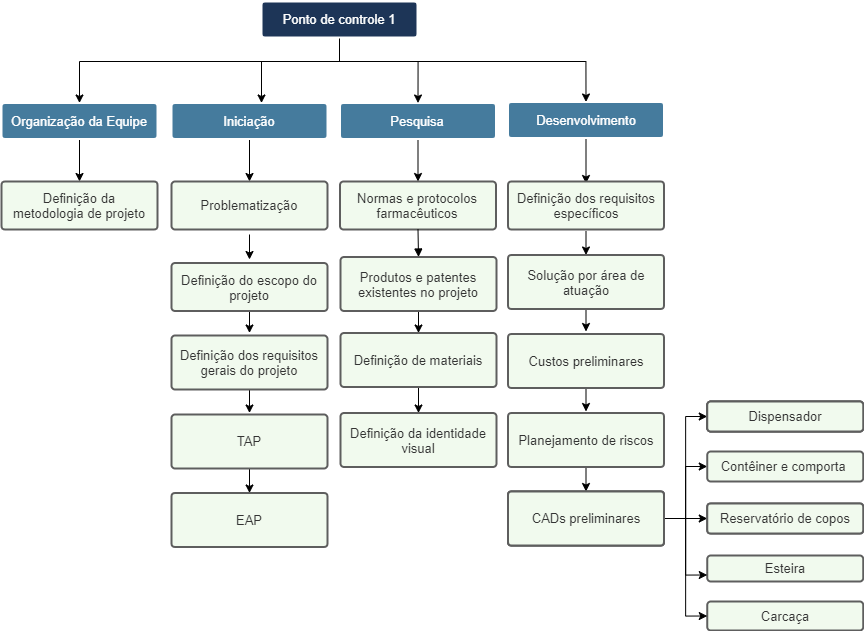
\includegraphics[width=\textwidth]{figuras/eap_pc1.png}
    \caption{Estrutura Analítica do Projeto PillWatcher - Ponto de Controle 1 }
    \label{fig:eap_pc1}
\end{figure}

\begin{figure}[H]
    \centering
    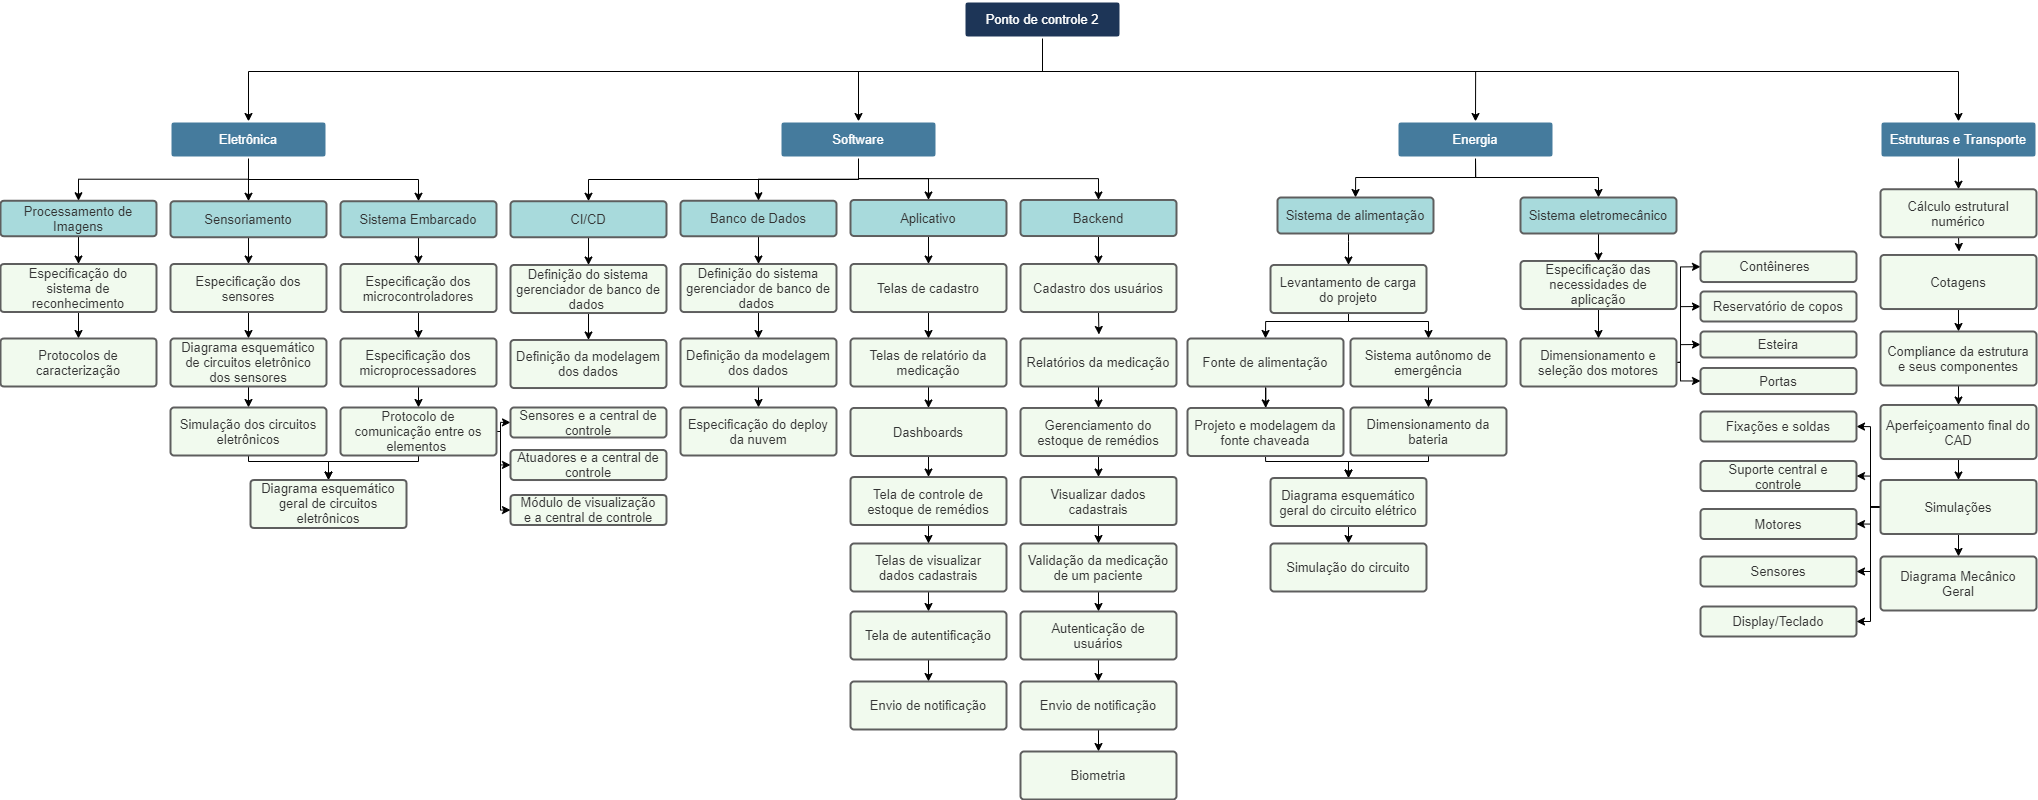
\includegraphics[scale=0.35, angle=90]{figuras/eap_pc2.png}
    \caption{Estrutura Analítica do Projeto PillWatcher - Ponto de Controle 2 }
    \label{fig:eap_pc2}
\end{figure}

\begin{figure}[H]
    \centering
    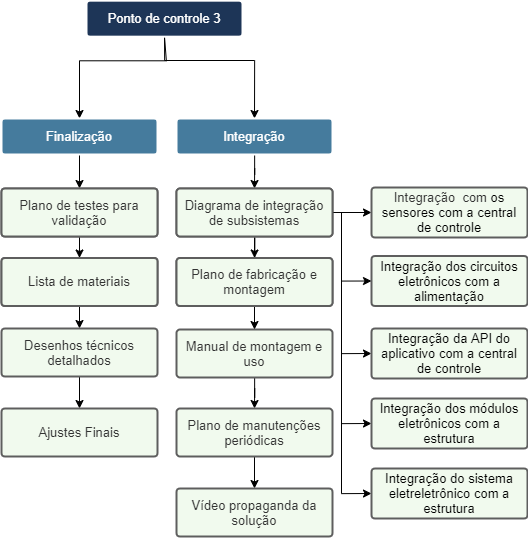
\includegraphics[width=0.7\textwidth]{figuras/eap_pc3.png}
    \caption{Estrutura Analítica do Projeto PillWatcher - Ponto de Controle 3 }
    \label{fig:eap_pc3}
\end{figure}

\begin{figure}[H]
    \centering
    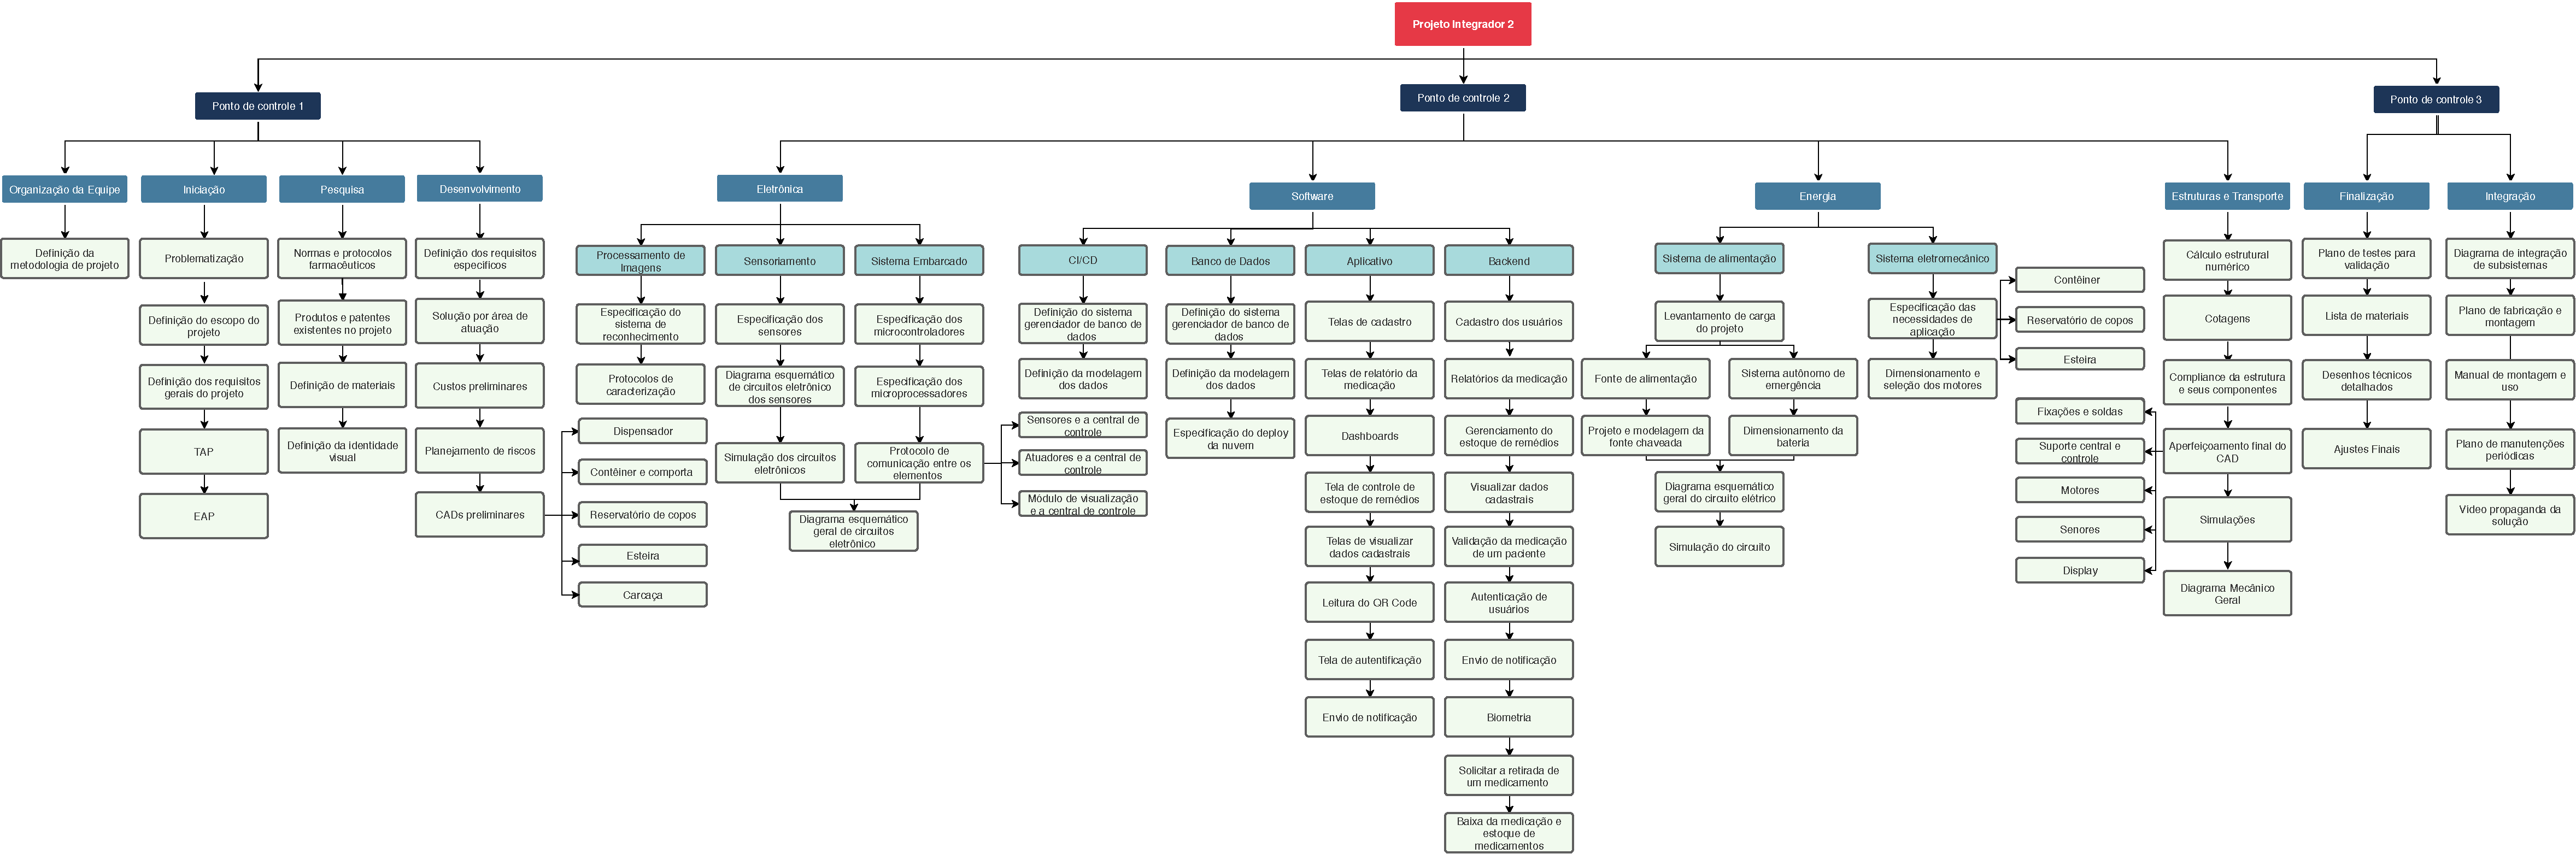
\includegraphics[scale=0.31, angle=90]{figuras/EAP.pdf}
    \caption{Estrutura Analítica do Projeto PillWatcher}
    \label{fig:EAP}
\end{figure}


%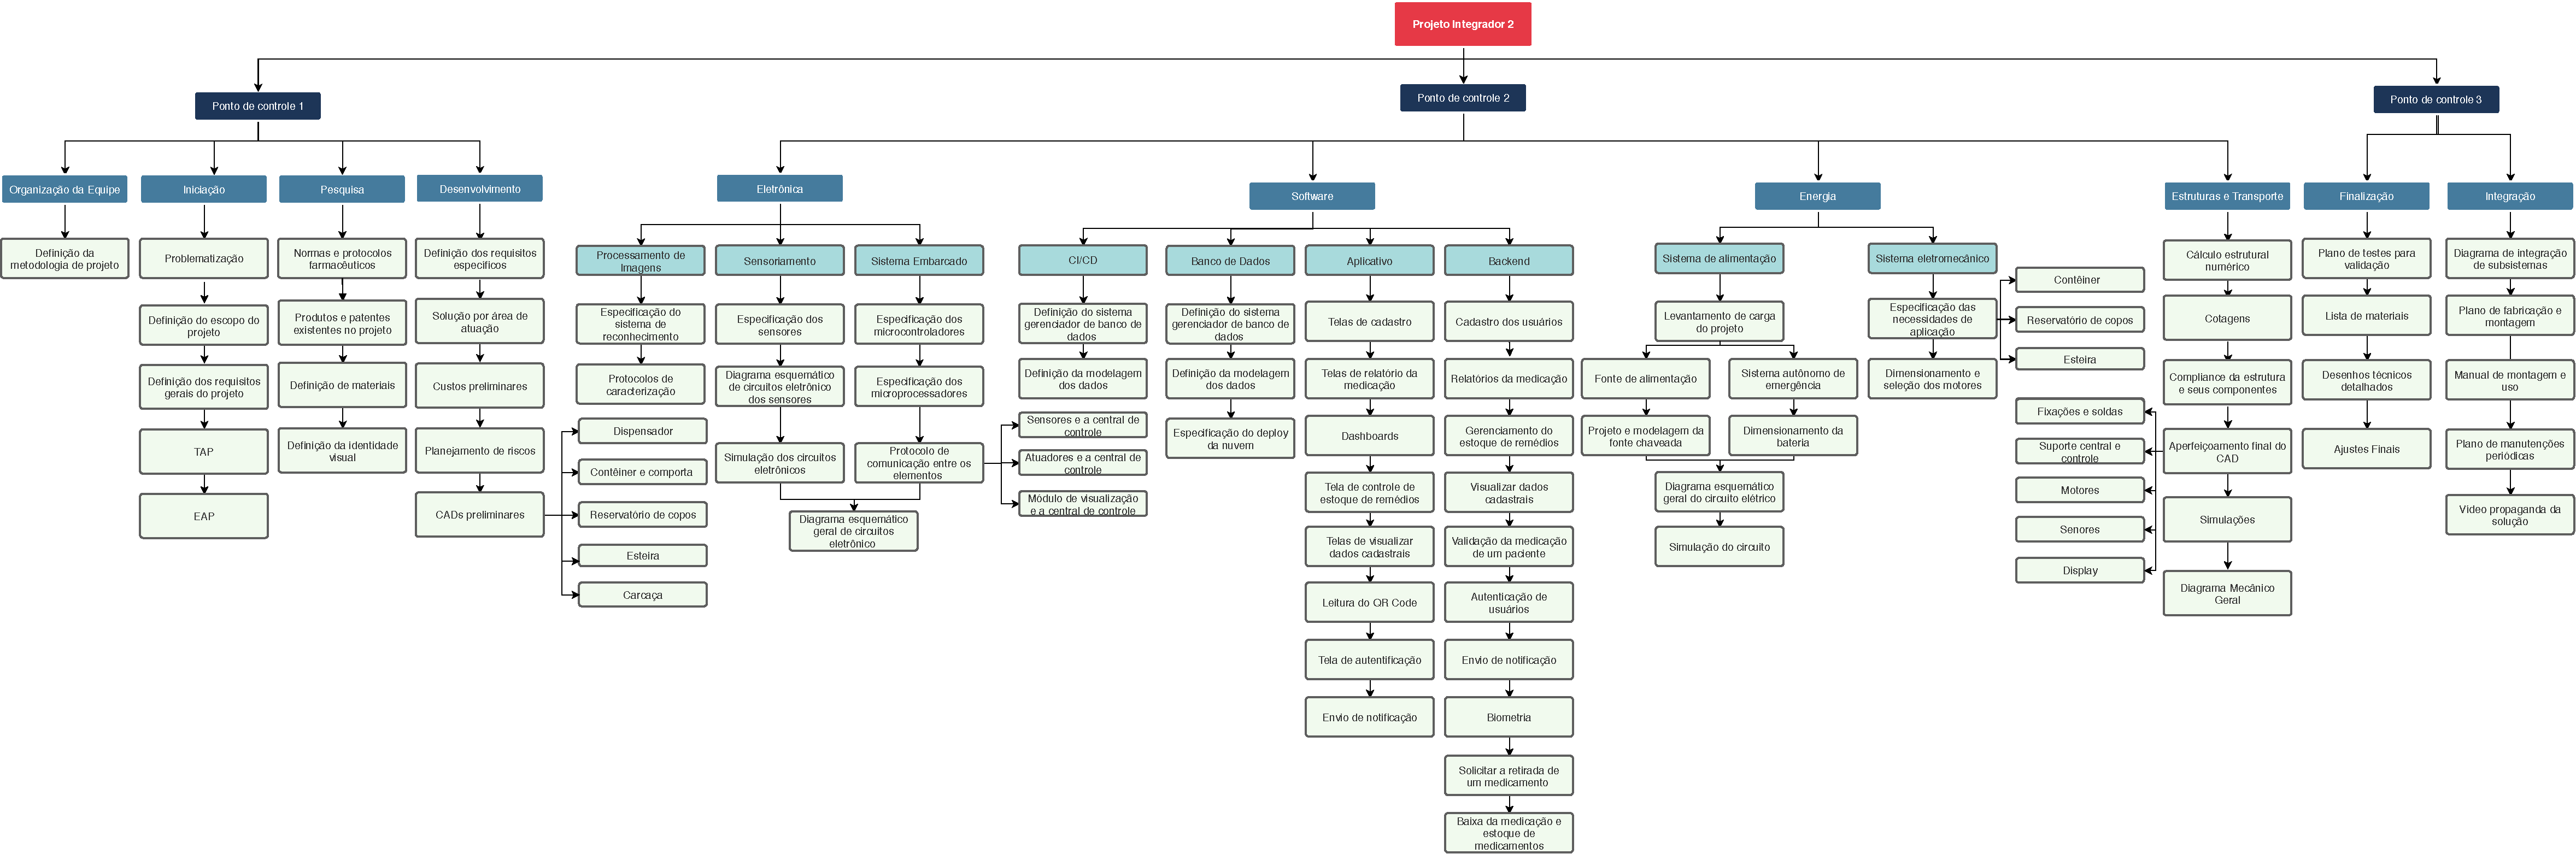
\includepdf[scale=0.73,angle=90,pages=1,pagecommand=\label{EAp}, offset=1cm -1.5cm]{figuras/EAP.pdf}

\chapter{Lista É/ Não É}
\label{Lista_app}

\begin{table}[H]
    \centering
    \caption{Lista É/Não é}
    \label{tab:lista_e_n_e}
    \begin{tabularx}{\textwidth}{|X|X|}
        \hline
        \rowcolor[HTML]{A8DADC}
        \multicolumn{1}{|X}{\textbf{É}} & \multicolumn{1}{|X|}{\textbf{Não é}} \\ 
        \hline
        1.1 É um sistema automático & 1.2 Não é um sistema autônomo \\ 
        \hline
        2.1 É um dispensador de medicamentos sólidos (comprimidos, drágeas e capsulas) & 2.2 Não é um dispensador de medicamentos líquidos, invetáveis ou pastosos \\ 
        \hline
        3.1 A quantidade de contêineres é pré-definida & 3.2 A quantidade de contêineres não é variável\\ 
        \hline
        4.1 Os contêineres recebem separadamente cada medicamento & 4.2 Os contêineres não armazenam doses de diferentes medicamentos \\
        \hline
        5.1 É um dispositivo que funciona interligado à rede elétrica & 5.2 Não é um dispositivo que deve funcionar desconectado da rede, salvo em falha da fonte primária \\ 
        \hline
        6.1 Para uso coletivo & 6.2 Para uso individual\\ 
        \hline
        7.1 Controlado via aplicativo & 7.2 Controlado manualmente via dispensador\\ 
        \hline
        8.1 Responsável por verificar se a medicação foi corretamente armazenada e separada em doses & 8.2 Responsável por ministrar a medicação\\ 
        \hline
        9.1 É um dispositivo fixo & 9.2 Não é um dispositivo transportável \\ 
        \hline
    \end{tabularx}
\end{table}

\chapter{Plano de Gerenciamento de Comunicação}
\label{Comunicação_app}
O desenvolvimento do projeto vigente requer o conhecimento de diversas áreas das engenharias envolvidas, sendo assim, o objetivo desse documento é padronizar as formas de comunicação interna entre os integrantes da equipe de projeto, bem como as ferramentas utilizadas para comunicação e gerência da equipe.

\section{Ferramentas}

\begin{table}[H]
    \centering
    \caption{Ferramentas de Comunicação}
    \label{tab:comunicacao}
    \begin{tabularx}{\textwidth}{|X|X|}
        \hline
        \rowcolor[HTML]{A8DADC}
        \multicolumn{1}{|c|}{\textbf{Ferramenta}} & \multicolumn{1}{|c|}{\textbf{Descrição}} \\ \hline
        \textit{Telegram} &  A ferramenta será utilizada para o compartilhamento de arquivos, links, marcar reuniões, alertas e discussões imediatas com a equipe. \\\hline
        Microsoft Teams &  A ferramenta será utilizada para fazer \textit{brainstorming}, \textit{sprint planning}, \textit{dailys} e reuniões mais extensas com todo o grupo para tirar dúvidas ou passar informações do projeto. Além de armazenar imagens e arquivos. \\\hline
        \textit{Github} & A plataforma será utilizada para centralização da documentação na \textit{Wiki} e onde será colocado os códigos produzidos pelas subequipes de Eletrônica e Software.\\ \hline
        \textit{Notion} & A ferramenta será utilizada para o mapeamento de tarefas, priorização e atualização de seu estado por parte das sub-equipes.  \\ \hline
        \textit{Overleaf} &  A ferramenta será utilizada para formatar e editar online os relatórios dos pontos de controle em LaTex. \\ \hline
    \end{tabularx}
\end{table}

\section{Diretrizes e Procedimentos de Comunicação}

Para manter uma boa comunicação entre as sub-equipes, as reuniões com todos os alunos do grupo de trabalho possuem horário fixo, segundas-feiras às 20:00h pelo {Microsoft Teams} e os \textit{Daily meeting} são realizados todos os dias pelo \textit{Telegram}.

Vale ressaltar que além dos horários de reuniões fixos, cada sub-equipe é responsável por verificar e estabelecer o melhor horário de reuniões por área, a qual a maioria dos integrantes estejam presentes.

\chapter{Plano de Gerenciamento de Recursos Humanos}
\label{RH_app}

\section{Papeis e Responsabilidades}
A partir da determinação da disciplina, a equipe será organizada de modo a existir os seguintes papéis: Coordenador Geral, Diretor de Qualidade, Diretores Técnicos e Time de Desenvolvimento.

\begin{figure}[H]
    \centering
    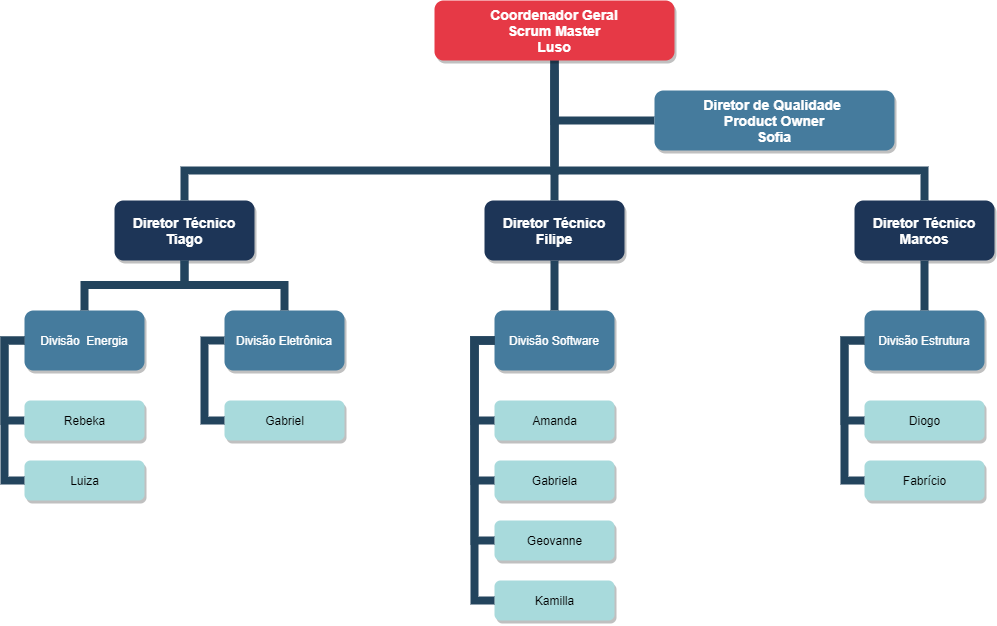
\includegraphics[width=0.9\textwidth]{figuras/div_papeis.png}
    \caption{Organograma da Divisão de Funções}
    \label{fig:papeis}
\end{figure}

\subsection{Coordenador Geral}
\begin{itemize}
    \item Controlar o cronograma e cumprimento das atividades no prazo;
    \item Validar e controlar o escopo do projeto, o plano de produção e integração em conjunto com os outros diretores;
    \item Manter todos os envolvidos informados a respeito do projeto;
    \item Atuar na definição e validação de requisitos técnicos, de forma a garantir que a arquitetura da solução atenda às necessidades do cliente.
\end{itemize}

\subsection{Diretor de Qualidade}
\begin{itemize}
    \item Controlar e validar o escopo do projeto;
    \item Garantir que os produtos desenvolvidos cumpram com os critérios de aceitação;
    \item Validar a usabilidade dos sistemas;
    \item Garantir a integração correta dos subprodutos;
    \item validação de documentação técnica do projeto;
\end{itemize}

\subsection{Diretor Técnico}
\begin{itemize}
    \item Gerenciar as atividades dos desenvolvedores e garantir a coesão do grupo;
    \item Atuar na definição de requisitos técnicos e tomada de decisão sobre tecnologias aplicáveis ao projeto e ao subsistema;
    \item Atuar na definição e aplicação de critérios de projeto, para garantir a correta especificação dos elementos;
    \item Atuar na validação de produtos dos desenvolvedores e garantir a interoperabilidade dos produtos entre subsistemas;
    \item Atuar na definição de planos de produção e integração entre produtos de diferentes equipes;
    \item Desenvolver e validar a documentação técnica da equipe;
\end{itemize}

\subsection{Desenvolvedor}
\begin{itemize}
    \item Identificar os requisitos técnicos e definição de tecnologias para resolver o problema abordado no projeto. A escolha das tecnologias deve ser justificada pelos desenvolvedores;
    \item Desenvolver e validar as partes técnicas sob sua responsabilidade;
    \item Definir critérios de produção e interoperabilidade dos produtos do seu subsistema;
    \item Desenvolver as documentações técnicas, referentes aos itens sob seu desenvolvimento.
    \item Participar da integração dos elementos de seu subsistema ao restante do projeto
\end{itemize}

\chapter{Cronograma por \textit{Sprint} e Ponto de Controle}\label{roadmap}

\vspace{-1.6cm}
\begin{figure}[H]
    \centering
    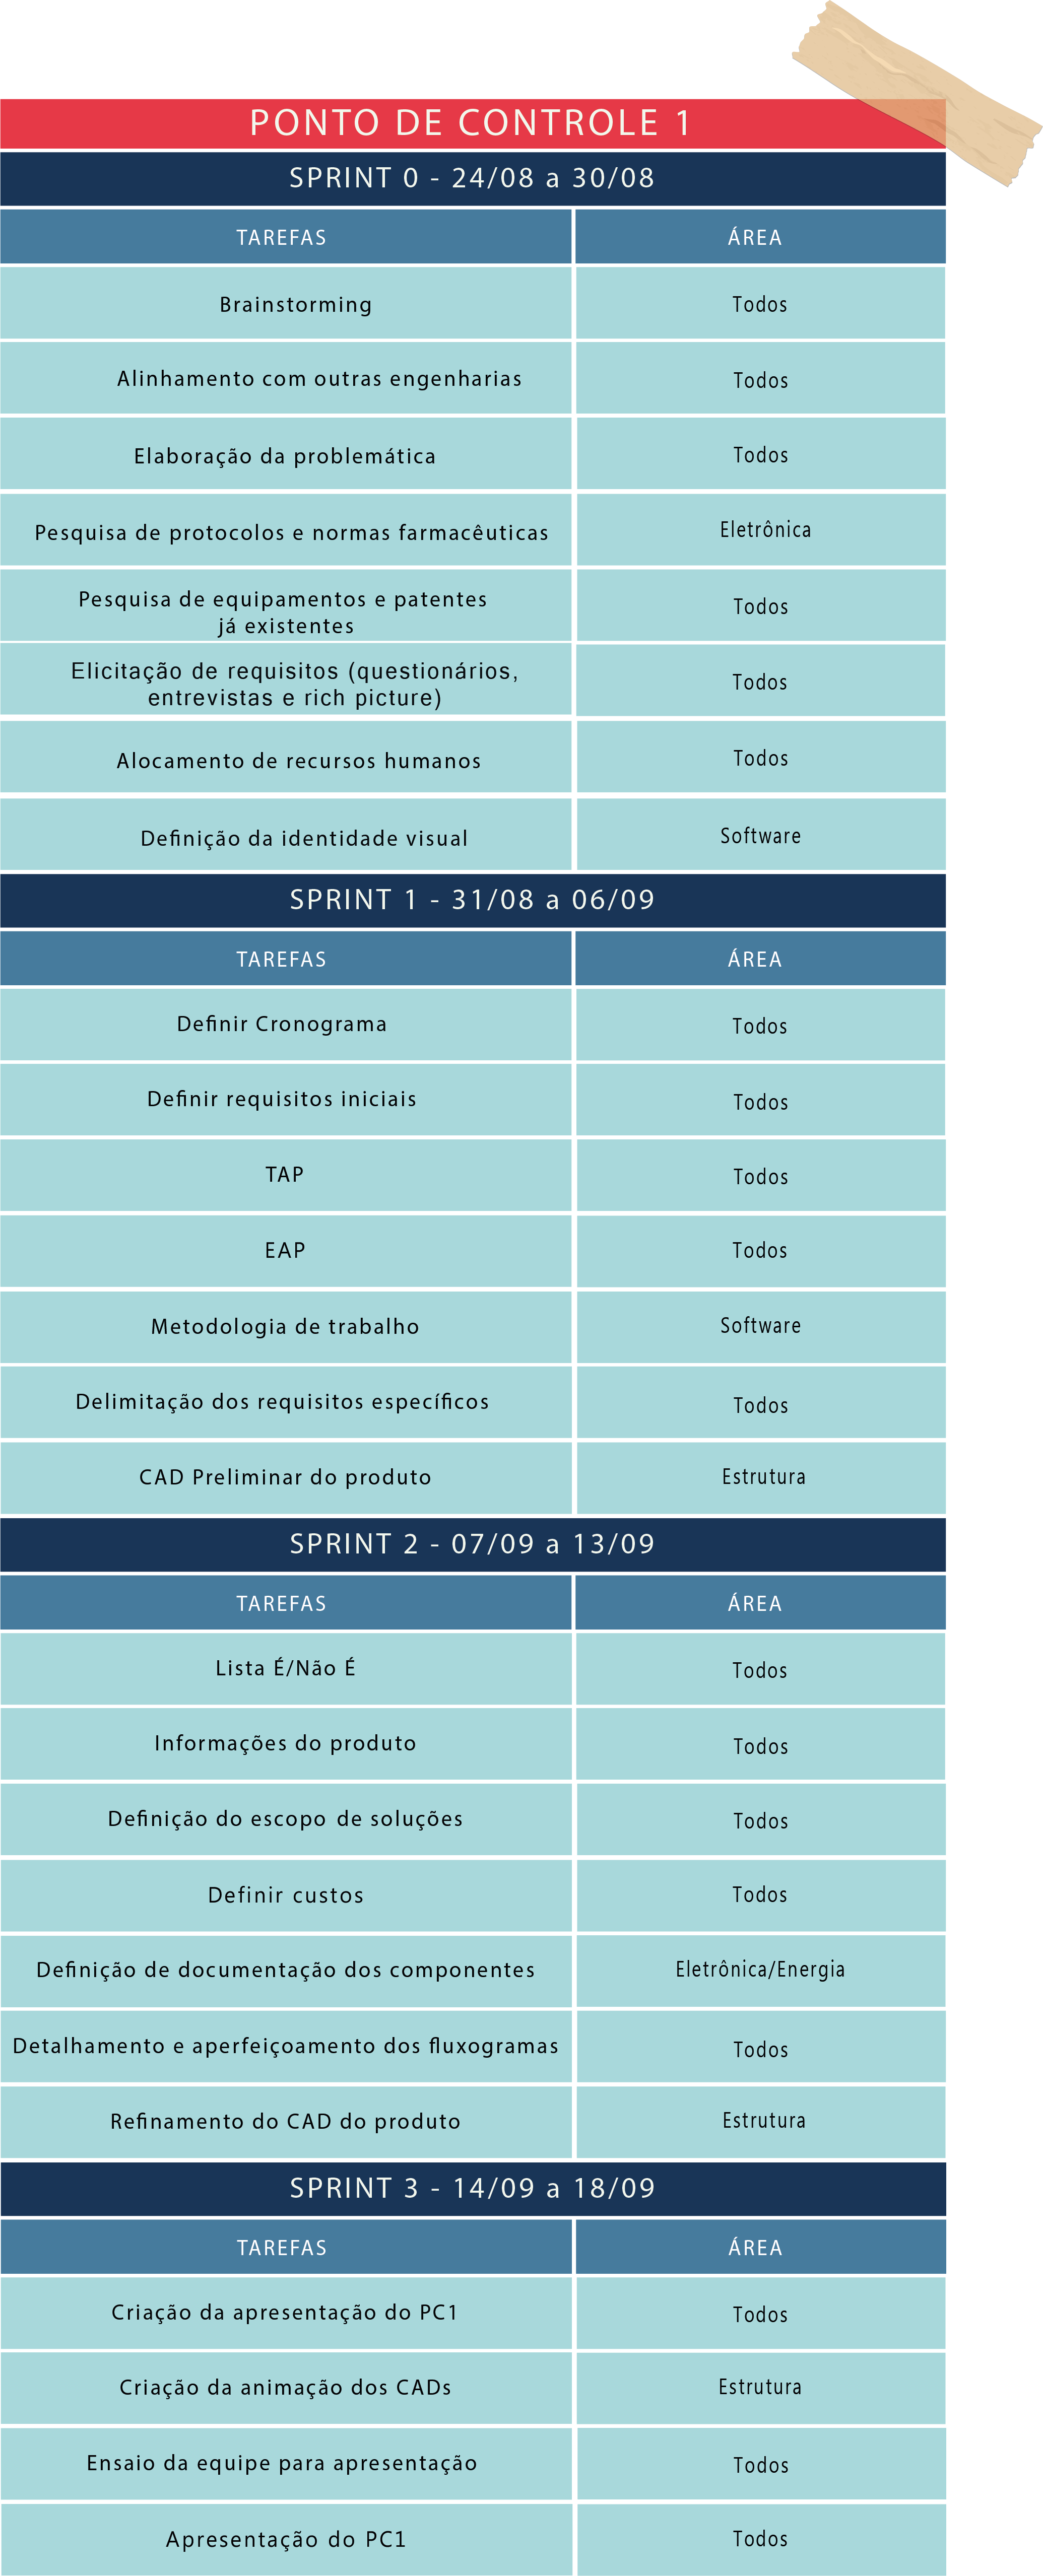
\includegraphics[width=0.5\textwidth]{figuras/sprint-pc1.png}
    \caption{Planejamento Ponto de Controle 1}
    \label{fig:Sprint_pc1}
\end{figure}

\begin{figure}[H]
    \centering
    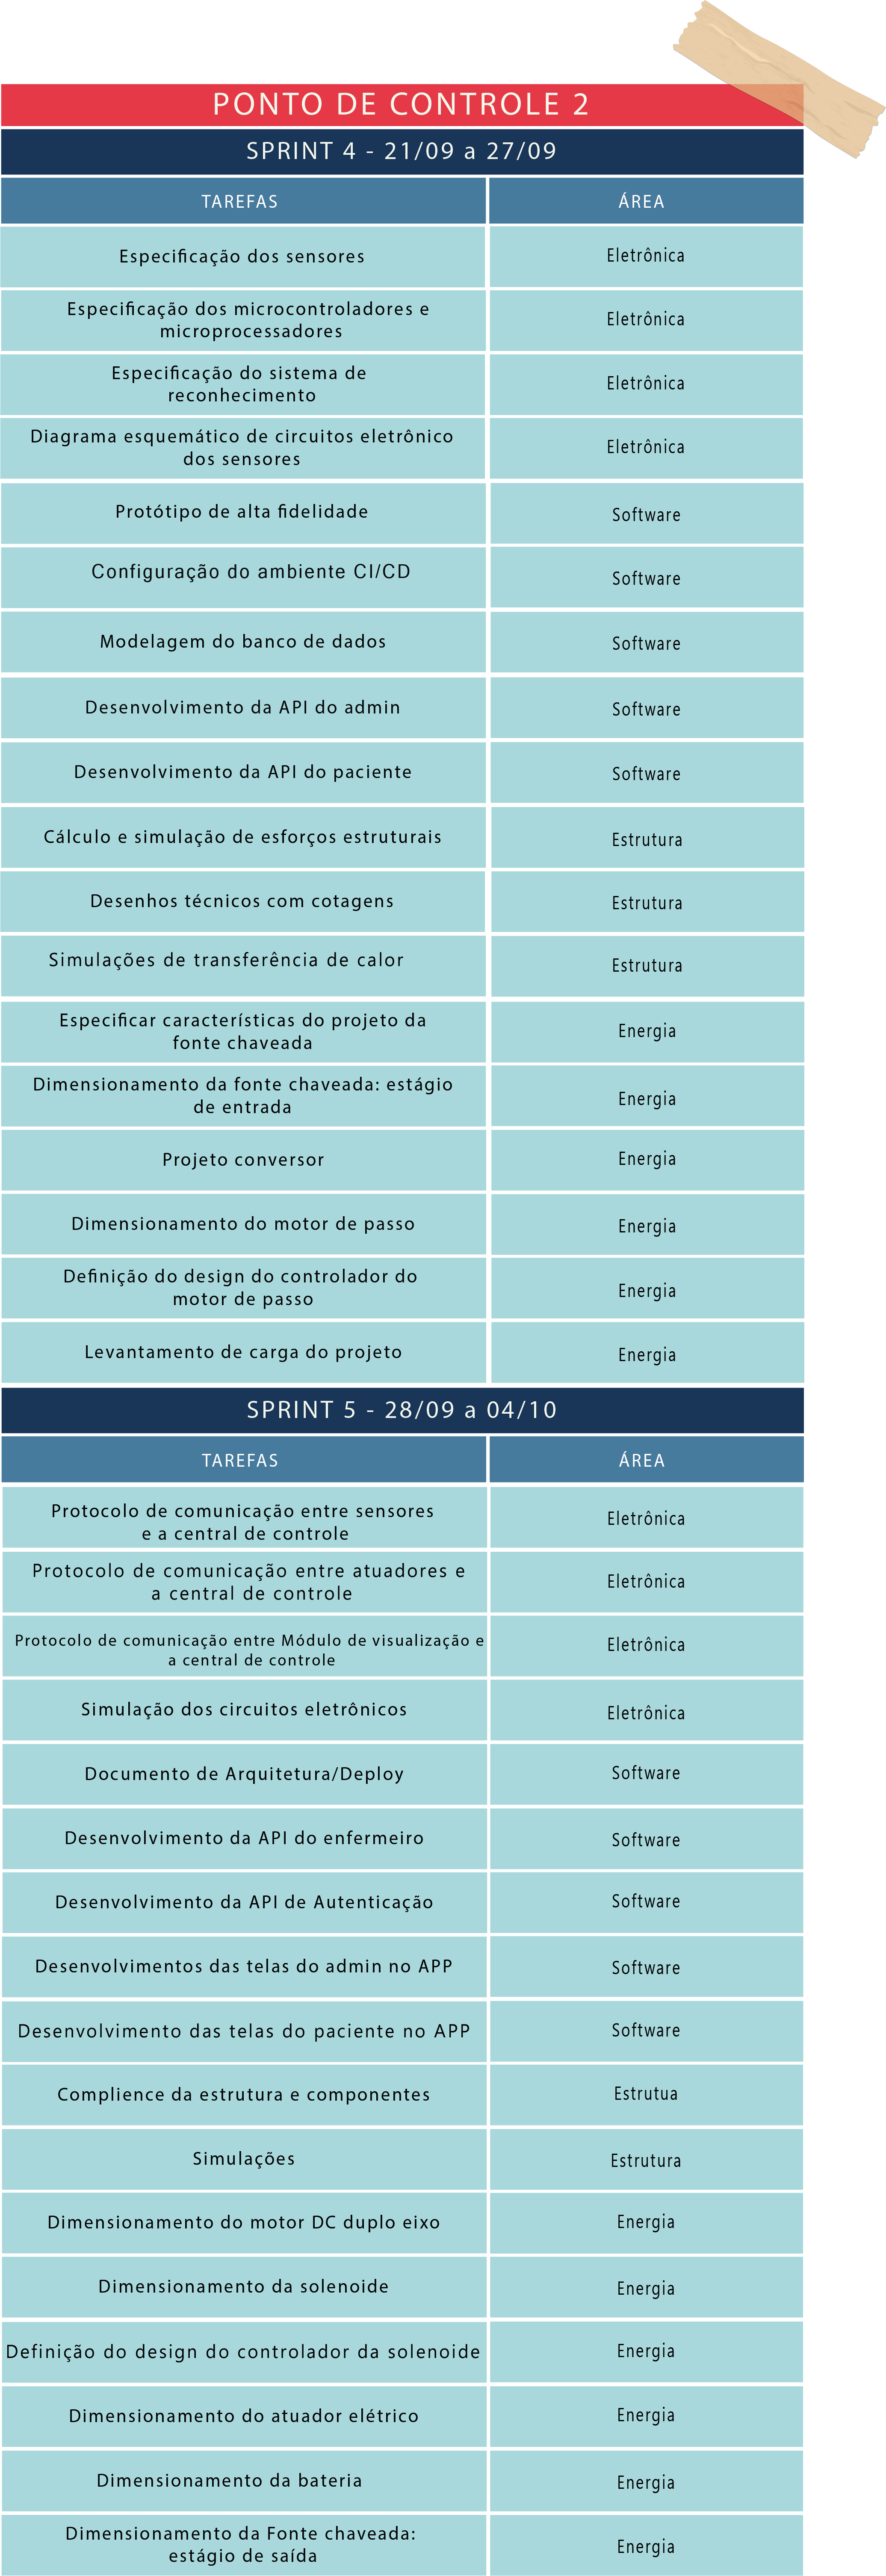
\includegraphics[width=0.5\textwidth]{figuras/sprint-pc2-1.png}
    \caption{Planejamento Ponto de Controle 2}
    \label{fig:Sprint_pc2}
\end{figure}

\begin{figure}[H]
    \centering
    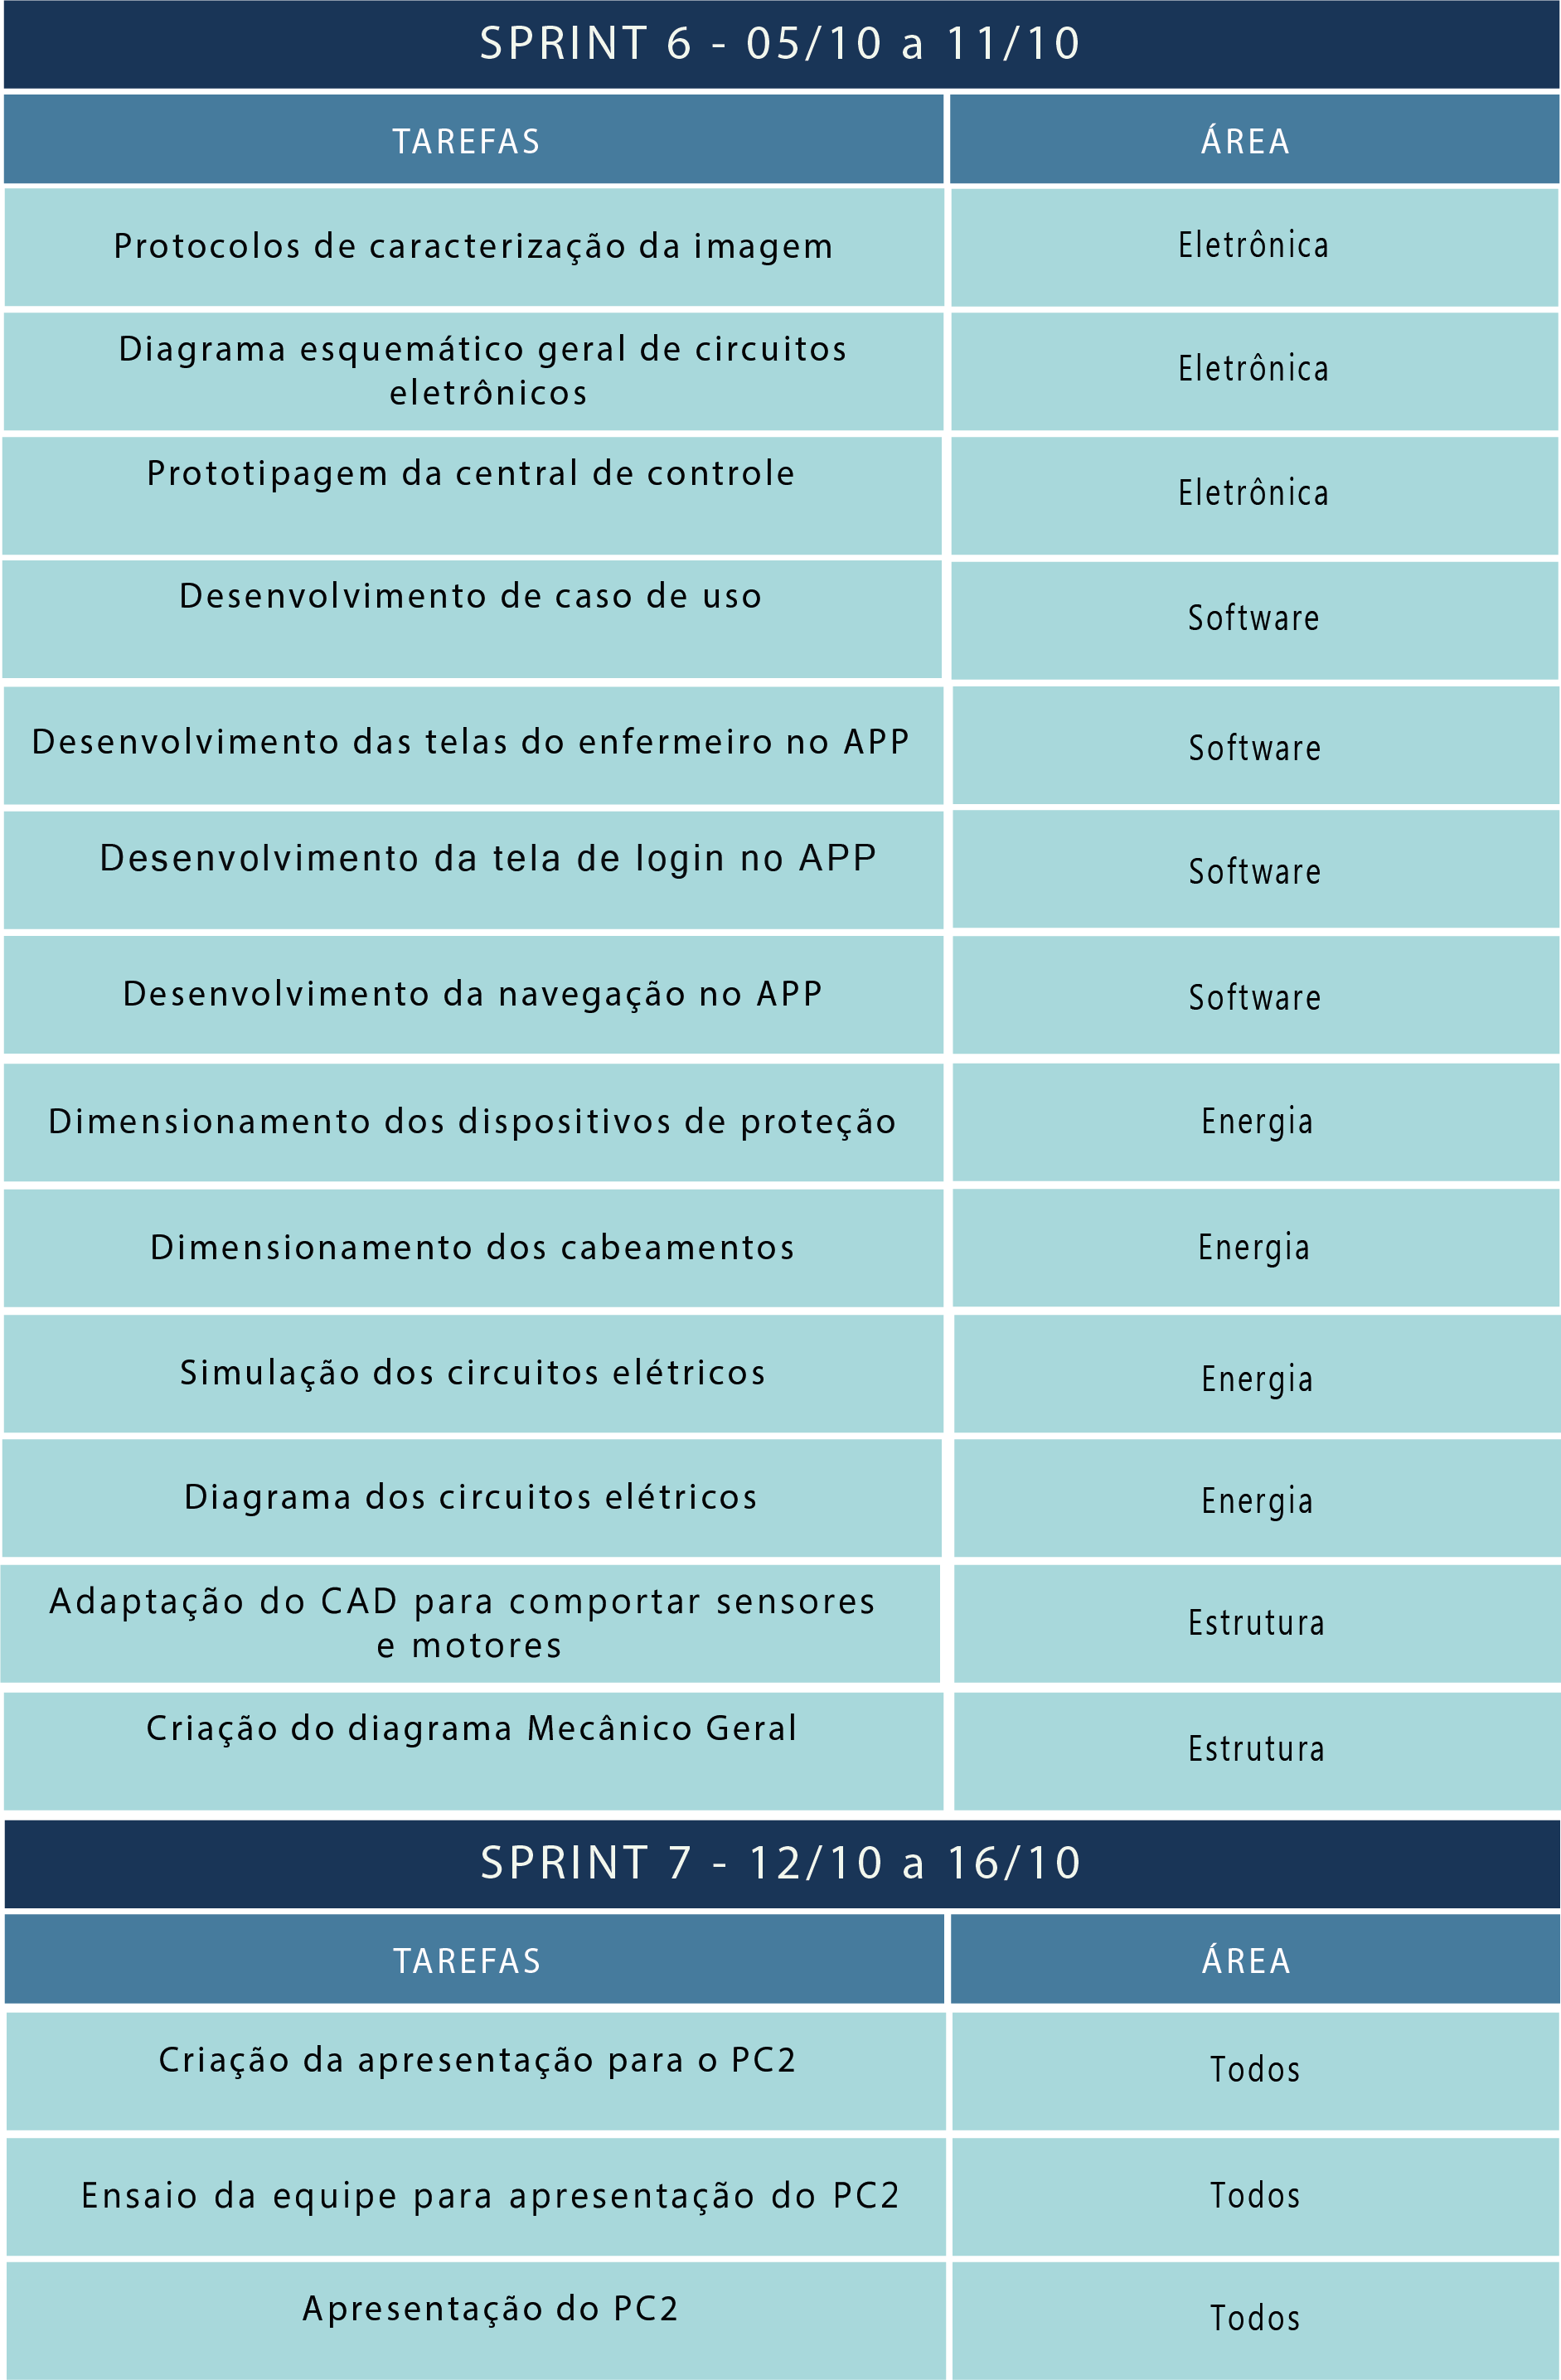
\includegraphics[width=0.5\textwidth]{figuras/sprint-pc2-2.png}
    \caption{Planejamento Ponto de Controle 2}
    \label{fig:Sprint_pc2_1}
\end{figure}

\begin{figure}[H]
    \centering
    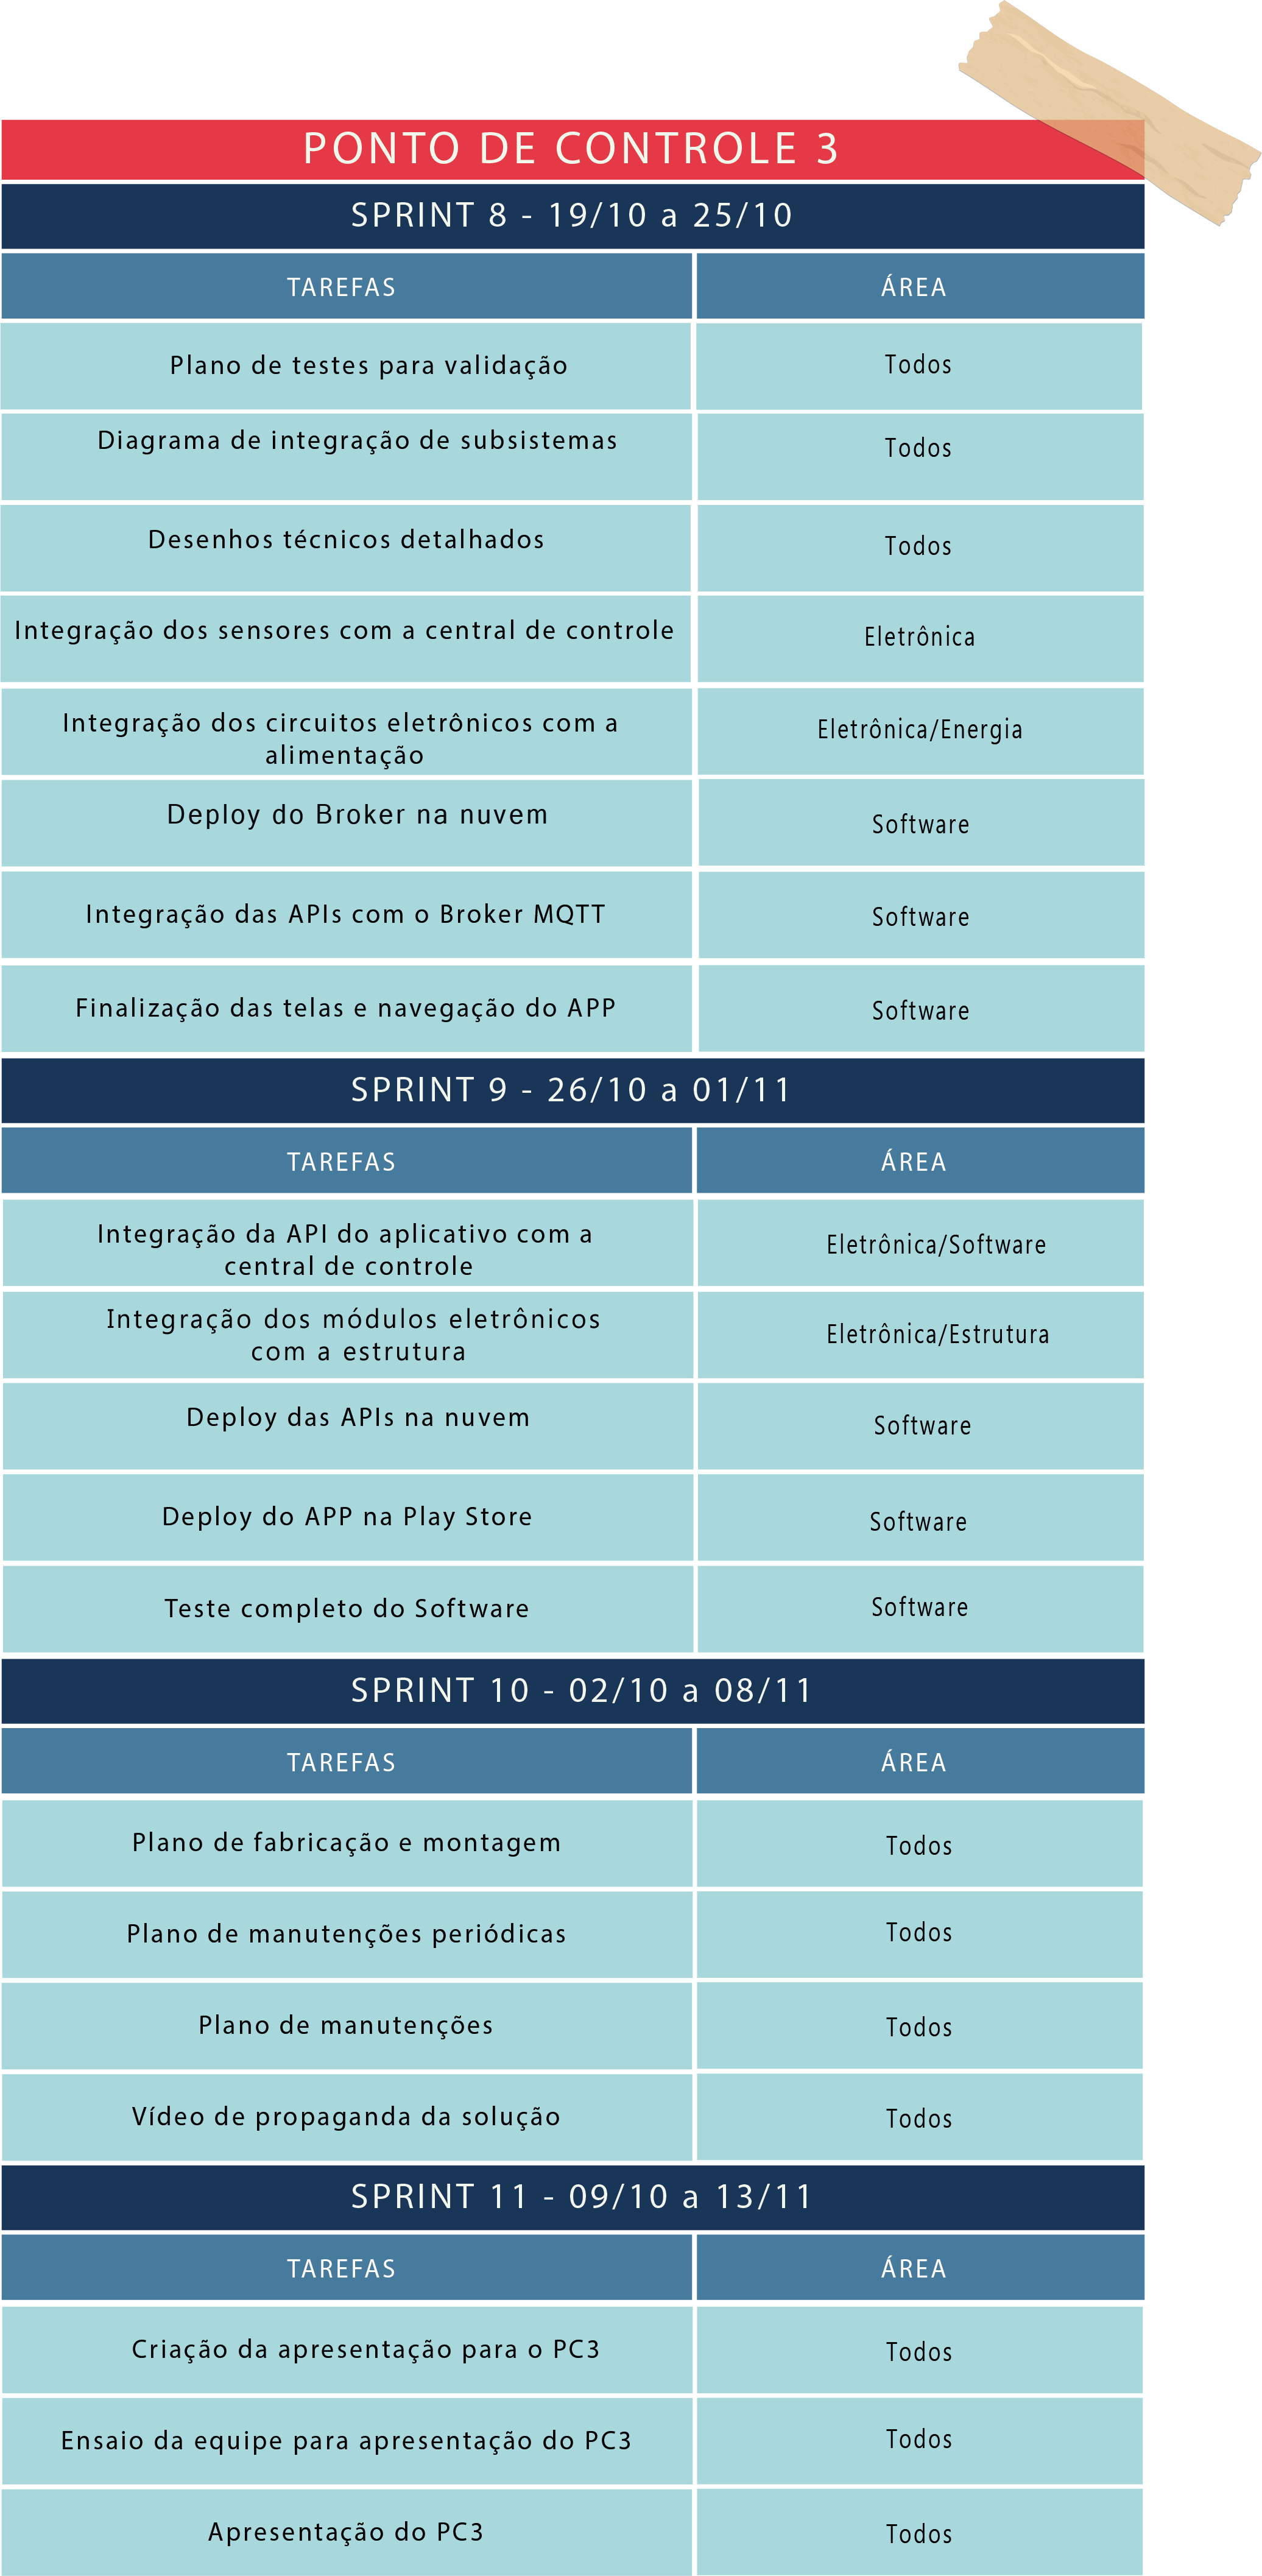
\includegraphics[width=0.5\textwidth]{figuras/sprint-pc3.png}
    \caption{Planejamento Ponto de Controle 3}
    \label{fig:Sprint_pc3}
\end{figure}

%% Rich Picture
\chapter{Rich Picture}
\label{richpiture_software}

\section{Comunicação Entre Componentes}
\begin{figure}[H]
    \centering
    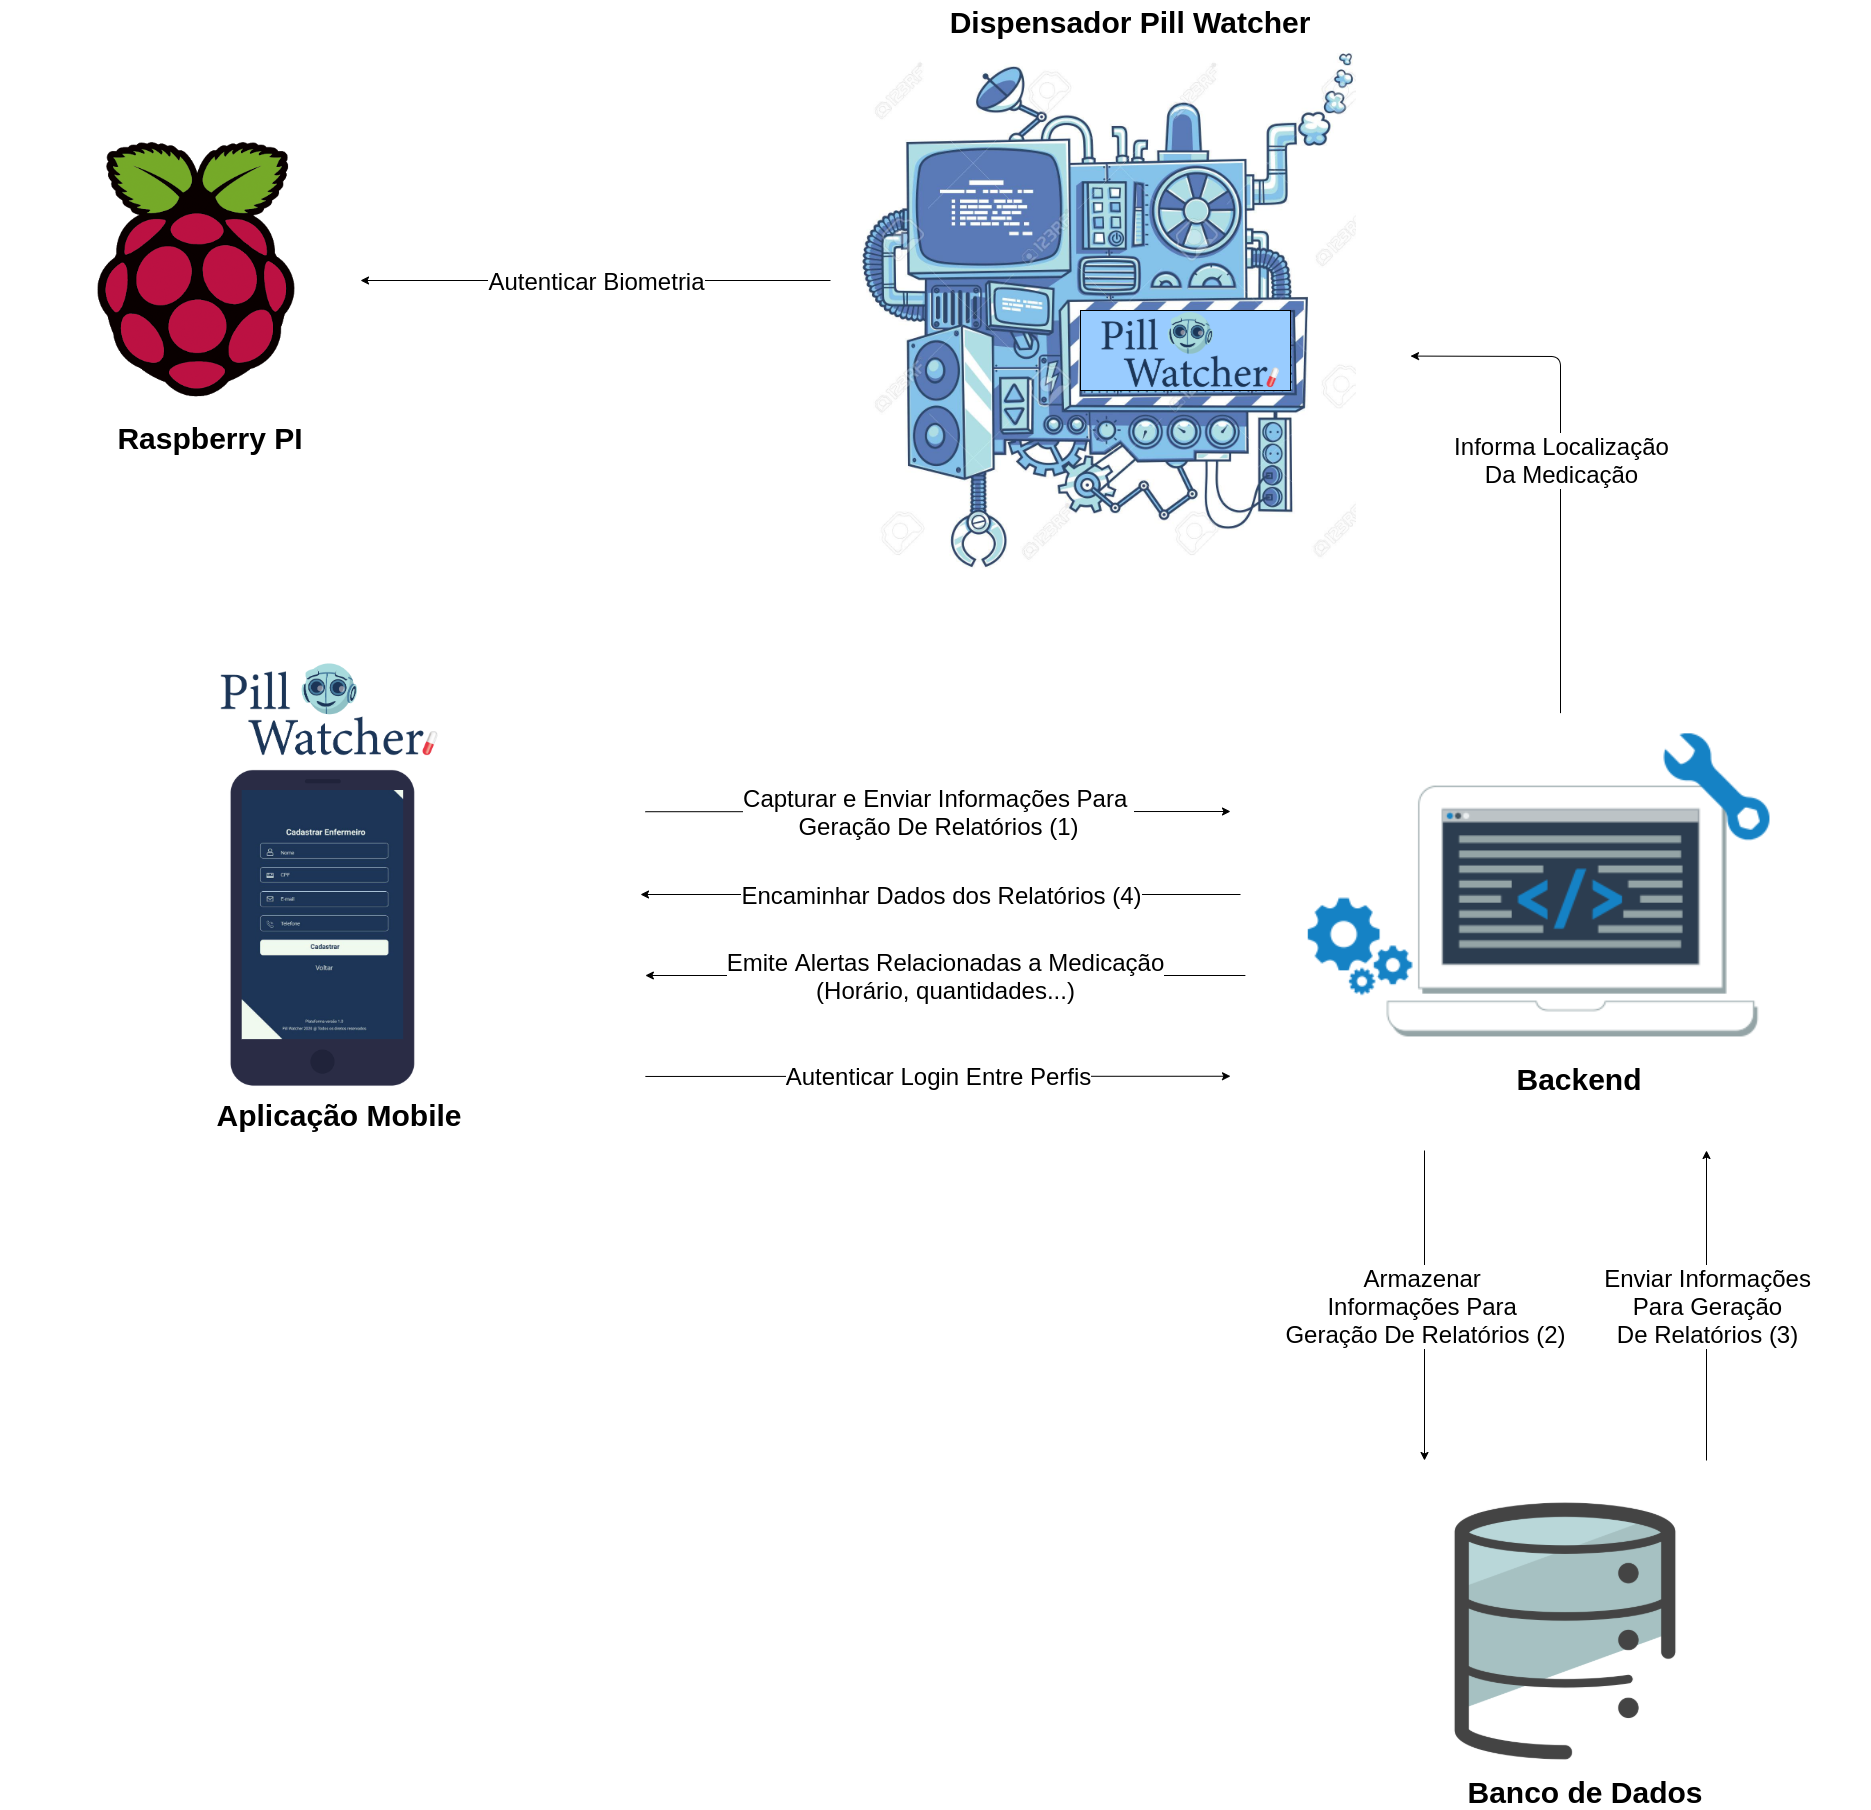
\includegraphics[width=1.0\textwidth]{figuras/Comunicação Entre Componentes.png}
    \caption{Comunicação entre componentes de software e eletrônicos}
    \label{fig:Communication_between_components}
\end{figure}

\section{Comunicação Entre Entidades e Solução de Software}
\begin{figure}[H]
    \centering
    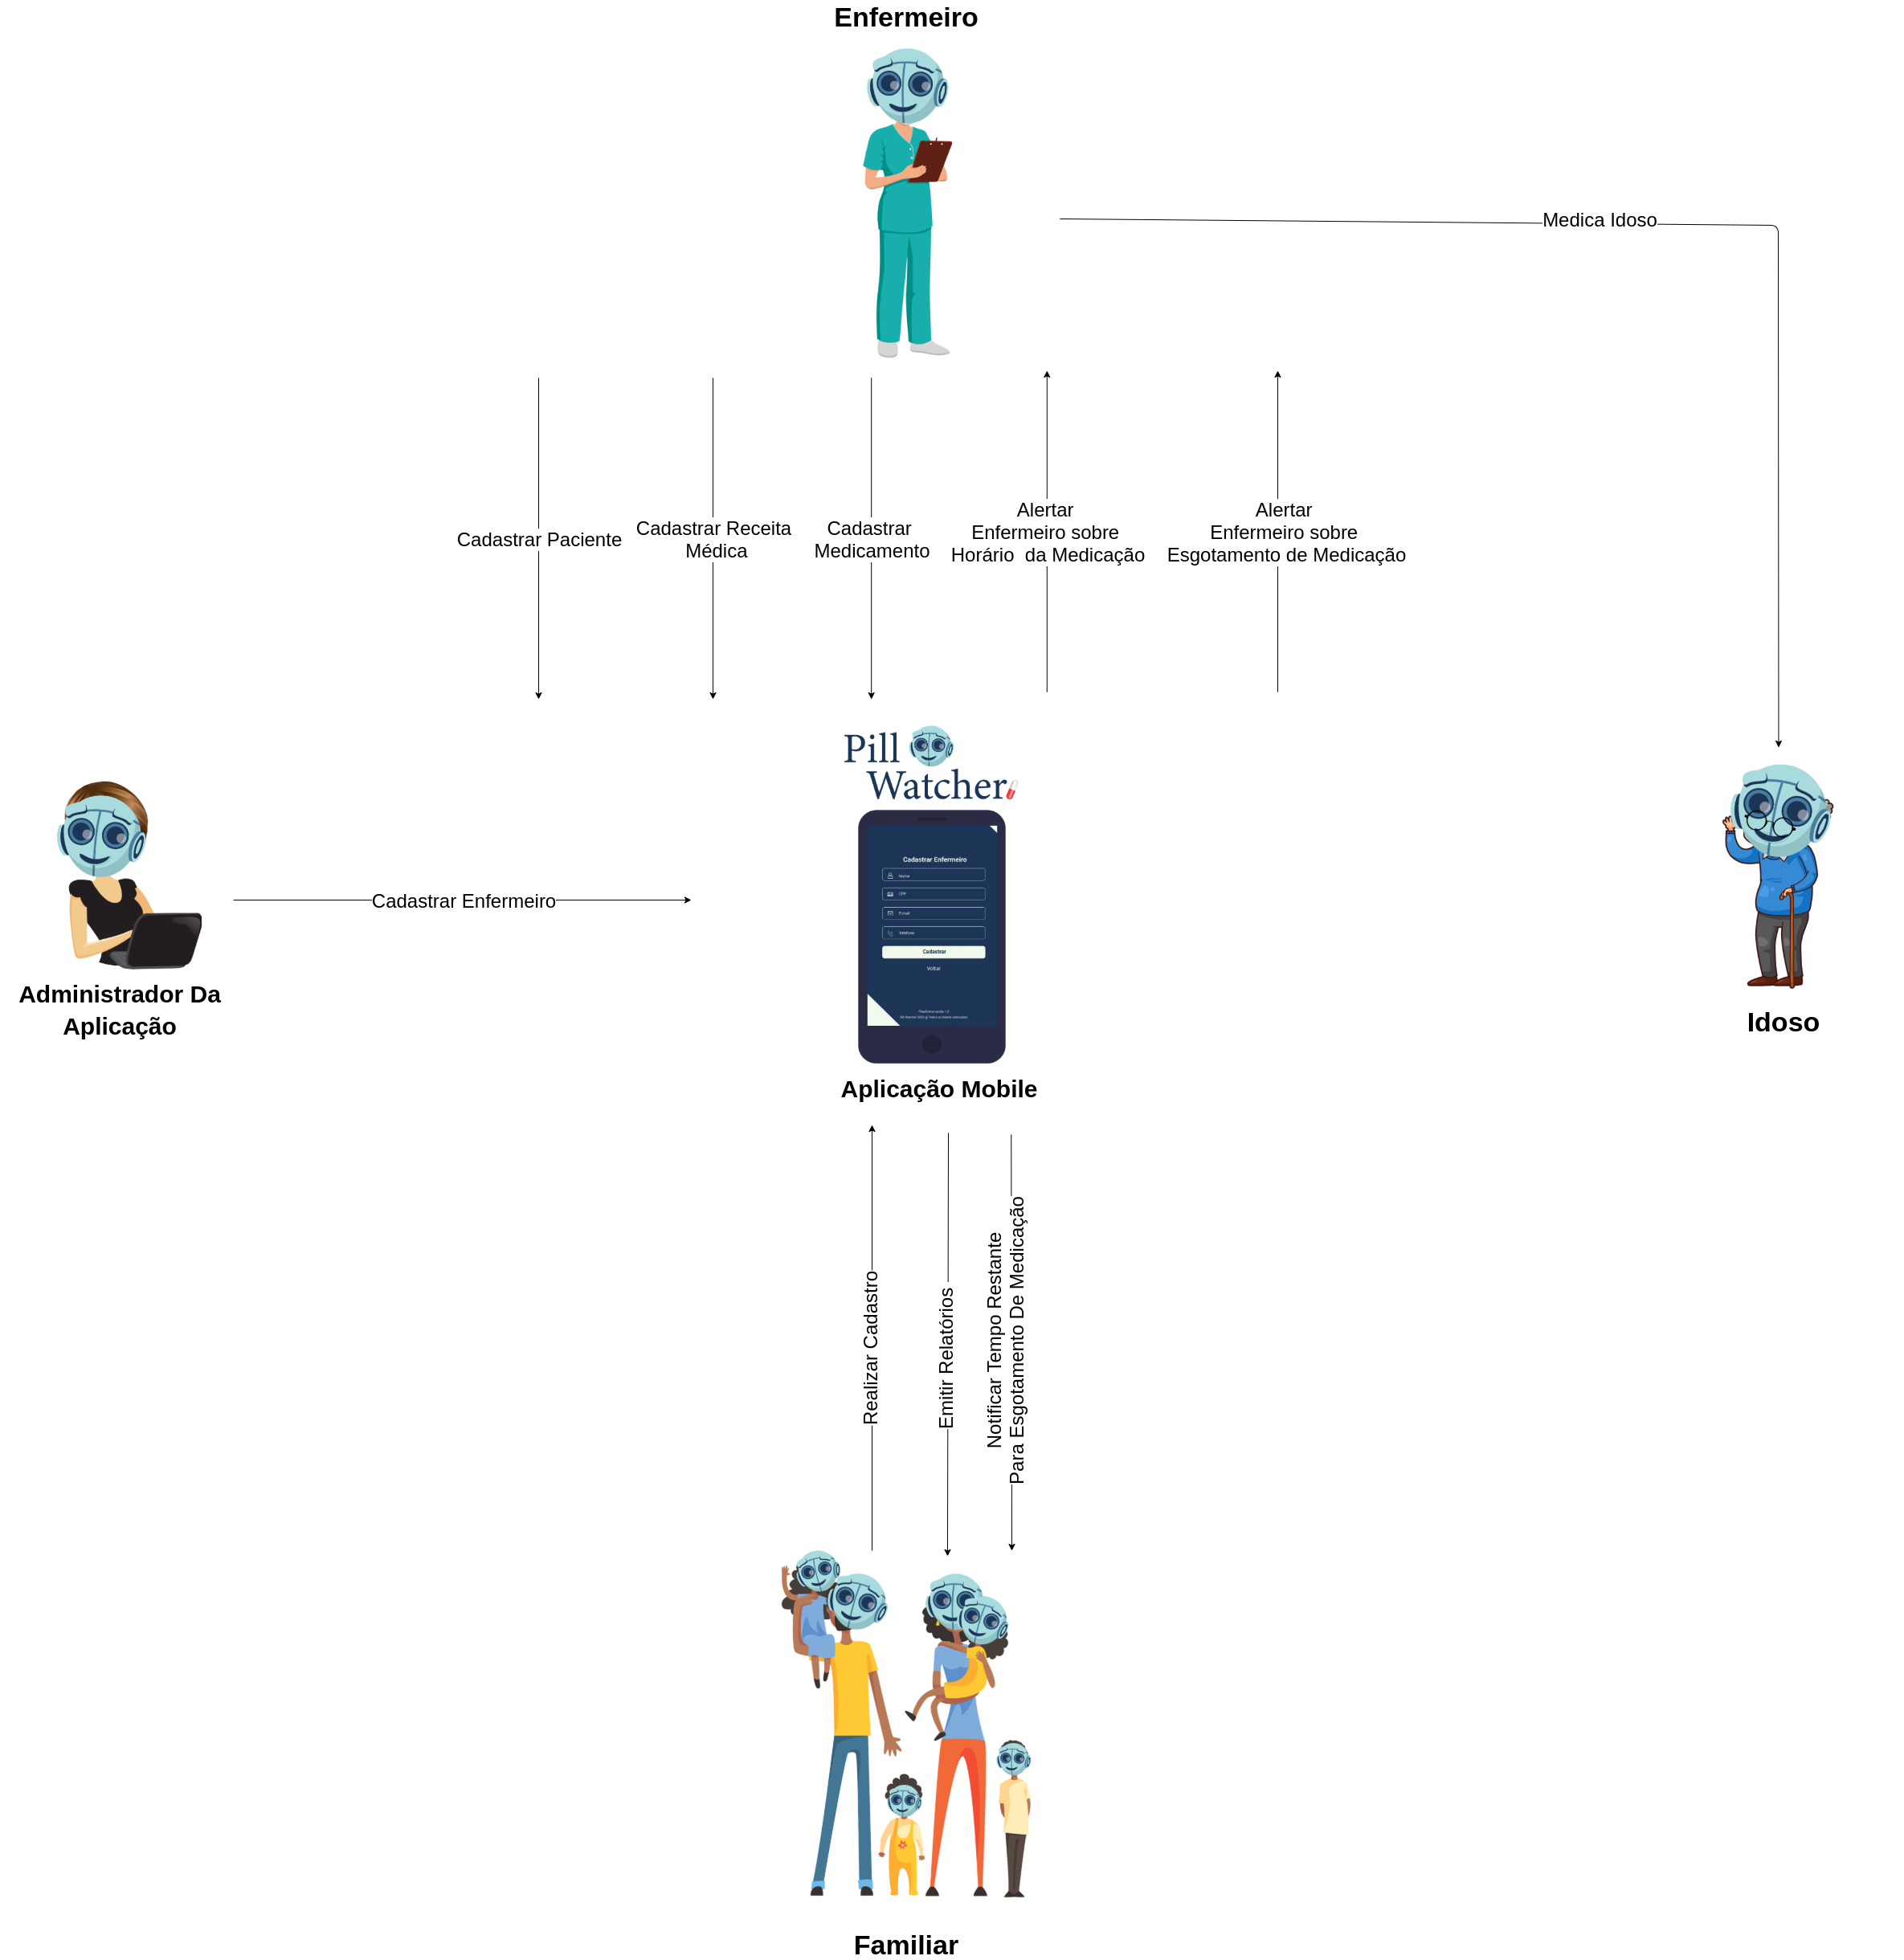
\includegraphics[width=0.9\textwidth]{figuras/Comunicação Entre Entidades e Solução De Software.png}
    \caption{Comunicação Entre Entidades e Solução de Software}
    \label{fig:Communication_between_entities}
\end{figure}

% CADs Preliminares
\chapter{Desenhos Técnicos Preliminares}\label{cad_preliminar}


\begin{figure}[H]
    \centering
    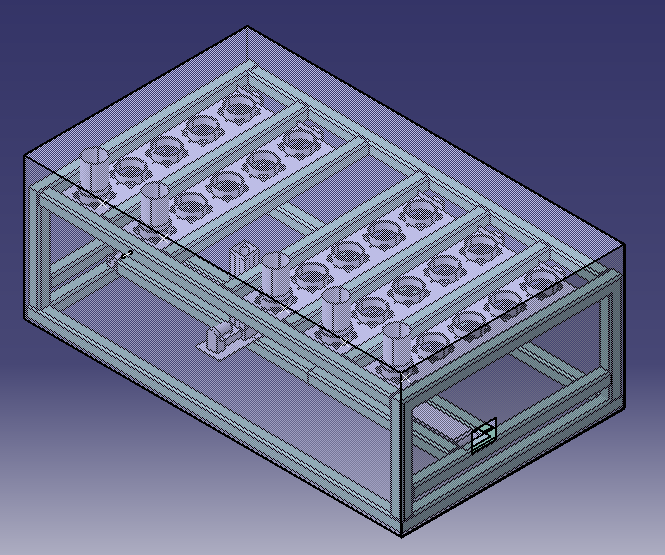
\includegraphics[width=0.7\textwidth]{figuras/estrutura/Global.png}
    \caption{Estrutural Global}
    \label{fig:global}
\end{figure}

\begin{figure}[H]
    \centering
    \includegraphics[width=0.7\textwidth]{figuras/estrutura/Carcaça.png}
    \caption{Carcaça da estrutura}
    \label{fig:Carcaca}
\end{figure}

\begin{figure}[H]
    \centering
    \includegraphics[width=0.7\textwidth]{figuras/estrutura/Porta de saída.png}
    \caption{Porta de saida}
    \label{fig:portas}
\end{figure}

\begin{figure}[H]
    \centering
    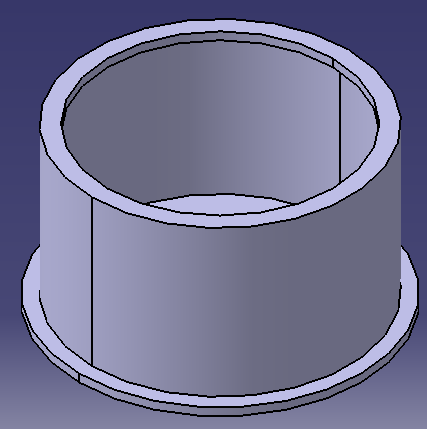
\includegraphics[width=0.7\textwidth]{figuras/estrutura/Copo.png}
    \caption{Ilustração do Copo}
    \label{fig:copos}
\end{figure}

\begin{figure}[H]
    \centering
    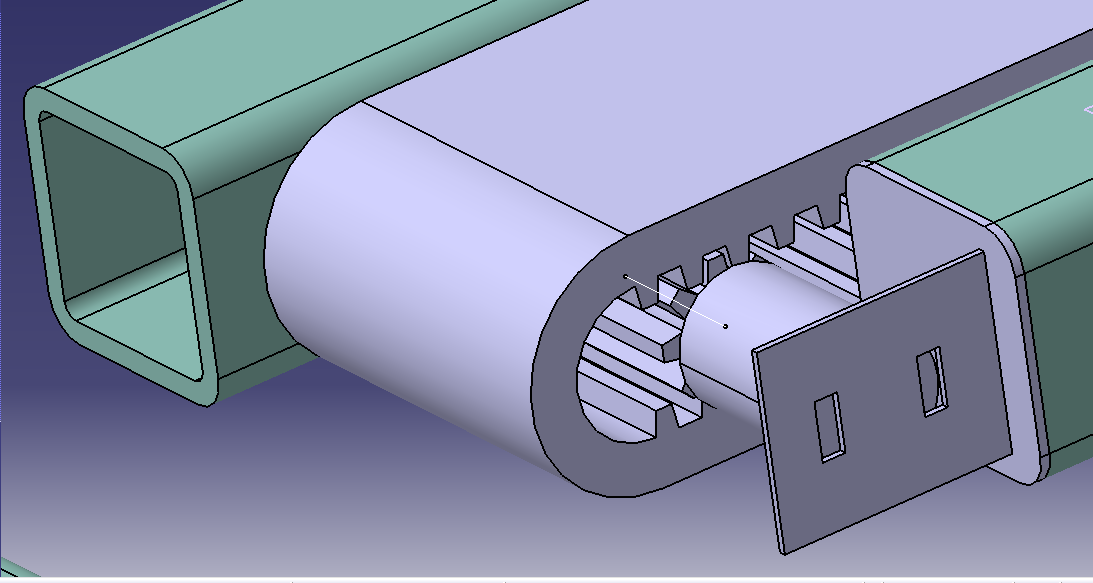
\includegraphics[width=0.9\textwidth]{figuras/estrutura/Motor DC na Esteira.png}
    \caption{Motor DC na esteira}
    \label{fig:DCnaesteira}
\end{figure}

\begin{figure}[H]
    \centering
    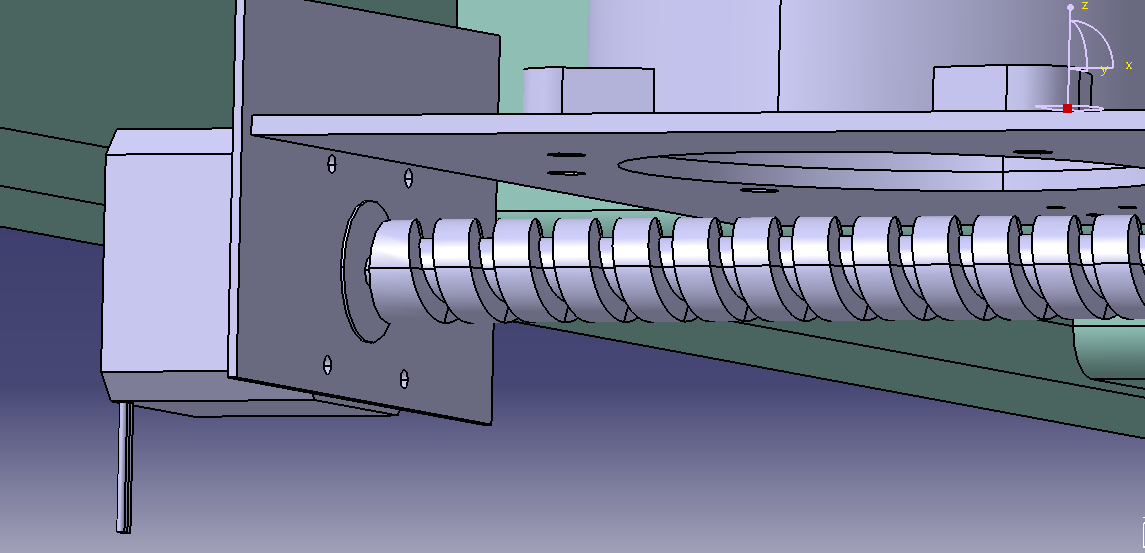
\includegraphics[width=1\textwidth]{figuras/estrutura/Motor de Passo no Fuso.png}
    \caption{Motor de passo com fuso}
    \label{fig:motordepassonofuso}
\end{figure}

\begin{figure}[H]
    \centering
    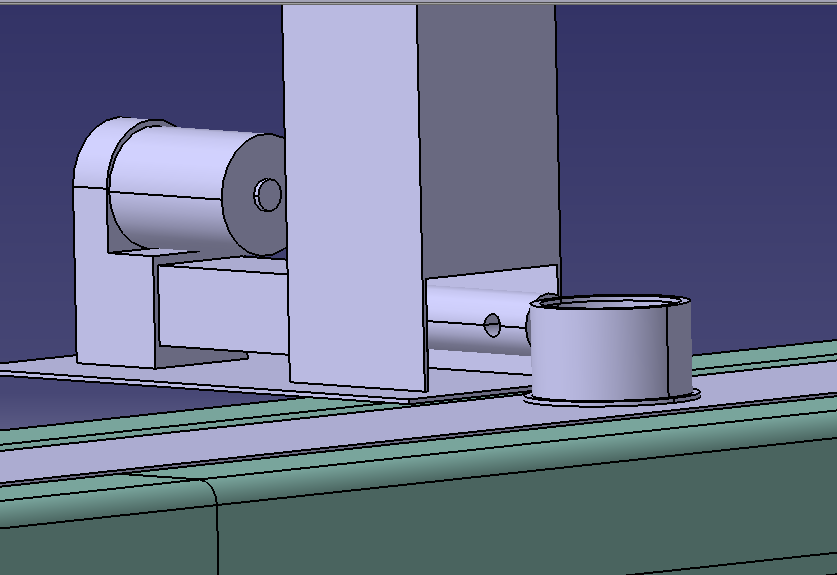
\includegraphics[width=0.9\textwidth]{figuras/estrutura/Recipiente dos Copos + Esteira.png}
    \caption{Reservatório de copos com esteira}
    \label{fig:reservatorioCopos}
\end{figure}

\begin{figure}[H]
    \centering
    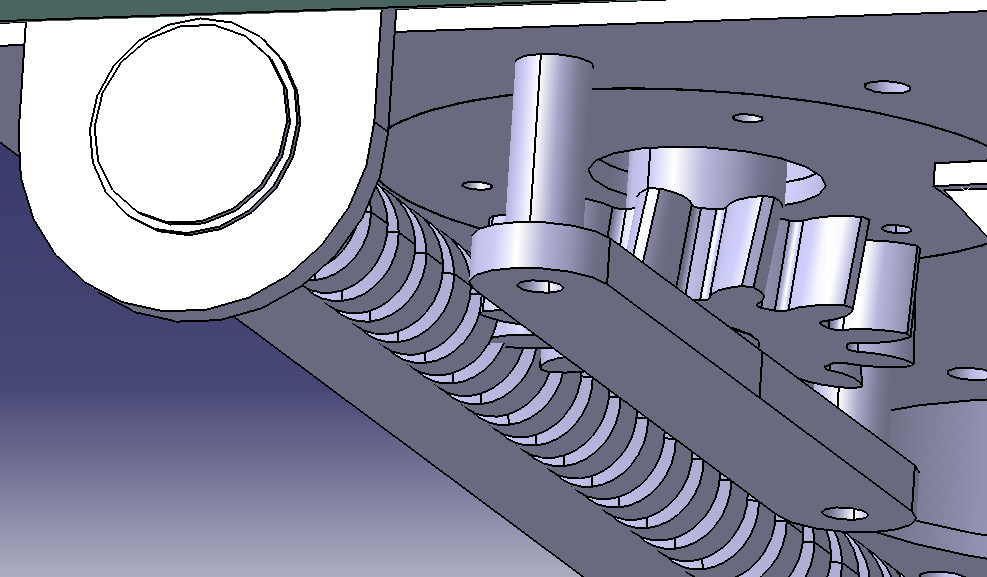
\includegraphics[width=0.9\textwidth]{figuras/estrutura/Detalhe Fuso com Engrenagem.png}
    \caption{Detalhes do fuso com engrenagens}
    \label{fig:fusoEngrenagens}
\end{figure}   

\begin{figure}[H]
    \centering
    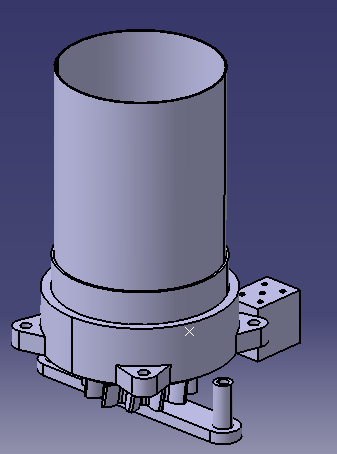
\includegraphics[width=0.7\textwidth]{figuras/estrutura/Conteiner.png}
    \caption{Contêiner dos medicamentos}
    \label{fig:conteiner}
\end{figure}

\begin{figure}[H]
    \centering
    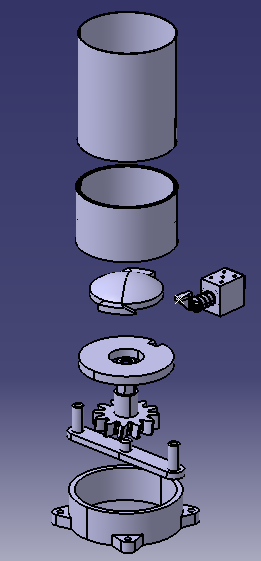
\includegraphics[width=0.6\textwidth]{figuras/estrutura/Descrição Contêiner.png}
    \caption{Descrição detalhada do contêiner}
    \label{fig:DescricaoConteiner}
\end{figure}

\begin{figure}[H]
    \centering
    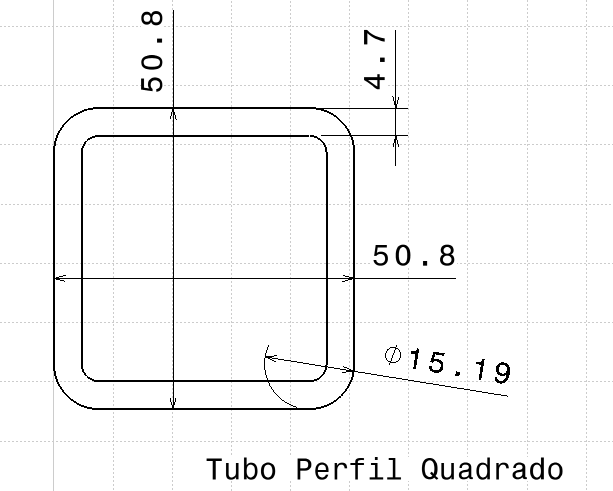
\includegraphics[width=0.8\textwidth]{figuras/estrutura/Perfil Quadrado.png}
    \caption{Cotagem do Tubo}
    \label{fig:Cotastubo}
\end{figure}    

\chapter{Entrevista com o Farmacêutico}\label{entrevista_app}

Foi realizada uma entrevista com farmacêutico Darlan Rodrigo da Silva.

\begin{enumerate}
\item \textbf{(Sofia) Existem padrões para dimensão de medicamentos? Qual órgão regulamenta? Quais são as medidas mais comuns?}

\textbf{(Farmacêutico)} Os medicamentos sólidos podem ser divididos em: comprimidos, capsulas e drágeas. Sendo assim, de comprimidos a Novalgina de 1g é a que possui maior diâmetro no mercado, já capsula gelatinosa é um pouquinho maior porem é mais maleável que o comprimido e varia de acordo com o objetivo de sua utilização como por exemplo: O local de absorção (sublingual que precisa ser absorvido rapidamente e que devido a esse fator é uma medicação muito sensível a umidade). O comprimido que não é revertido, apenas feito na compressora de medicação é suscetível a umidade e possuem uma absorção mais lenta devido ao fato de ter sido desenvolvido para ser dissolvido no fim do trato gastrointestinal e absorção do princípio ativo. A escolha do formato envolve a marketing utilizada pela empresa (se será redondo, encapsulado ou não, a cor da medicação...). Logo eu não diria que existe uma medida específica, pois é muito variável e não existe uma especificação que regularmente um padrão mais ligado a cosmética das medicações.

\item \textbf{(Sofia) Existe um tamanho máximo do medicamento para ocorrer a deglutição?}

\textbf{(Farmacêutico)} Por exemplo a capsula, ela é um pouquinho maior e muito maior que aquelas capsulas como a de omeprazol ou de manipulação em que se faz muito encapsulamento, maior que estas eu nunca vi. Existe uma vitamina que é muito utilizada por gestante chamada Teri da Bayes que possui um formato elíptico, pouco maior que uma capsula, mas bem maleável. Mas raramente vai ter uma medicação com tamanho maior que de uma capsula, o que você vai ter é uma variação nos formatos. Mas agora o que vocês podem fazer é com base na capsula, tirar um tamanho máximo.

\item \textbf{(Sofia) Nós podemos retirar medicamentos que estejam no blister ou em frascos?}

\textbf{(Farmacêutico)}  Existem algumas farmácias que fazem a desblistagem (retirada do medicamento do blister). O blister ele é um dispositivo de armazenagem bastante seguro contra a umidade pois duas coisas com que o medicamento sofre muito e que deve ser tomado cuidado é a umidade e a temperatura. A umidade é devido ao fato de que se você deixar entrar umidade nele, ele esfarela depois. O recomendado é deixar em um local com temperatura de no máximo 30ºC e em ambiente fora de umidade. Não teria problema você retirar ele, o problema é onde ele ficará armazenado depois. Então no caso do projeto de vocês que se baseia em colocar em um novo recipiente separado, que esse recipiente possa ser bastante vedado medicamente, e que não permita entrada de umidade, que seja algo bem vedado mesmo e ai não terão problema com relação a afetar a medicação com fatores externos (umidade e temperatura). 

\item \textbf{(Sofia) Quanto tempo os medicamentos podem ficar fora da embalagem segundo os padrões de segurança?}

\textbf{(Farmacêutico)} Vai depender da validade do produto, contando que se tenha esse cuidado com a temperatura e umidade, ai vocês se baseiam pelo lote e validade dele.  

\item \textbf{ (Sofia) Para o manuseamento dos remédios no abastecimento do dispositivo, quais cuidados devem ser tomados para não haver contaminação?}

\textbf{(Farmacêutico)} É ai na questão de tirar do blister teria que ter todo um cuidado de manuseio da medicação, então nesse caso a deblistagem deveria ser realizada com cuidado, pois você esta retirando ele de um lugar limpo e fechado para um outro local que também deve estar esterilizado. Nessa transferência devem ser tomados esses cuidados (utilizando luvas, toucas, máscaras). Então talvez tenha que ser acompanhado de um procedimento para isso.

\item \textbf{(Sofia) Na bula da medicação é especificado se o medicamento é hidrofílico ou termolábil? Existem medicamentos sólidos Termolábeis?}

\textbf{(Farmacêutico)} Comprimidos orais quanto menos umidade e controle de temperatura de 15ºC até 30ºC está ok, mais que isso já podemos ter algum tipo de problema na medicação. Medicação com outras faixas de temperatura nos temos também que são refrigerados em temperatura de geladeira e com isso precisam ficar armazenadas nessa condição. Quais medicações são essas? Geralmente são medicações injetáveis, como vacinas, medicações para tratamento de câncer, dificilmente em comprimidos. Você pode observar na embalagem.

\item \textbf{(Sofia) Quais seriam os principais medicamentos e dosagens utilizados por pacientes de casa de repouso?}

\textbf{(Farmacêutico)} Essa pergunta já é muito específica específica, o que eu posso falar a respeito é que eu não sei exatamente qual a incidência de medicamento x ou Y em casas de repouso para idosos por exemplo, agora o que eu comento que acho que faria todo sentido, seria estudar as medicações utilizadas para o tratamento de doenças que afetam mais os idoso como: pressão alta, diabetes, sistema nervoso central, antidepressivos e medicação para dor. Então esse tipo de medicação eu acho que são bem comuns nesses locais


\item \textbf{(Sofia) Podemos utilizar o mesmo compartimento para um mesmo medicamento, mas para dois ou mais pacientes?}

\textbf{(Farmacêutico)} Olha, poderia misturar neste compartimento com alguns detalhes. Exemplo um compartimento com novalgina que tem que ser dada de 6 em 6 horas para seu João e Dona Maria. os medicamentos podem ficar juntos deste que sejam do mesmo lote e data de fabricação, pois se algum comprimido tiver algum problema você não consegue identificar o lote. Outro cuidado importante é saber se a dosagem que será armazena e a dosagem que o paciente precisará receber são as mesmas, uma vez que um medicamento pode ter mais de uma dosagem. 

\item \textbf{(Sofia) Após a utilização de um determinado compartimento por um determinado tipo de medicamento, existe a necessidade de higienização para um próximo medicamento?}

\textbf{(Farmacêutico)} Com certeza, isso é bem importante. Até na industria uma máquina de produção ela é utilizada para produzir vários medicamentos, porém é realizado uma limpeza completa do equipamento. E como eu garanto que a limpeza foi bem feita? a industria realiza vários testes. No dia dia nos também temos que ter esse cuidados, o comprimido vai soltando um pó, pode quebrar... Então pode ter alguns problemas. Com existem pessoas que são alérgicas a determinado tipo de medicação, isso é um problema ou pode sobrar um comprimido lá dentro. Então essa limpeza é extremamente relevante. Uma limpeza que garanta que não se tem mais resquícios da medicação anterior. Água e sabão podem resolver. Só tem que tomar cuidado com a umidade, o compartimento deve ser bem seco para não afetar o medicamento.

\item \textbf{(Sofia) Qual o melhor material para o compartimento de armazenamento dos comprimidos?}

\textbf{(Farmacêutico)} O inox é o melhor dos mundos, mas ele é caro e mais complicado de trabalhar que o plástico em si. Acho que tem farmácias que possuem umas caixinhas de plástico com repartições para você colocar horário, é feito de plástico. O inox visualmente e para limpeza é melhor, mas o plástico é tranquilo também até porque a medicação ficará ali só por alguns dias e logo vai acabar. Não sei se chegaram a pensar em algo que pode ser descartável, que pode ser destacado quando acabar ou algo assim. 

\item \textbf{(Sofia) Caso o medicamento não seja retirado do dispositivo no horário correto, qual o tempo máximo que pode ocorrer na administração da entrega dessa medicação?}

\textbf{(Farmacêutico)} Vai depender muito da medicação que a pessoa esta tomando e dos horários que ela toma. Cada fármaco tem um tempo de atuação no organismo, quando você ingere uma dipirona depois de 20 minutos á 30 minutos ela é absorvida no estomago e a dipirona entra na corrente sanguínea e ai o gráfico de concentração sanguínea da dipirona vai aumentando e atingir um pico máximo e depois vai descendo até ser eliminada. Antes dela ser eliminada você já administra uma outra dose para continuar com o efeito terapêutico dela, só que tem um detalhe, você precisa saber como funciona a curva para cada medicamento. Se você toma de 6 em 6 horas, depois de 6 horas como tá o nível de dipirona no organismo? está com feito terapêutico? sim, ainda não esta com febre. Agora quanto tempo mais eu posso ficar sem a dose para que n sinta as reações? Isso tem que ser avaliado pois não existe um padrão. Então é uma pergunta em que não temos como saber quanto tempo padrão para todos eles, e deve ser especificado em bibliografia para cada um deles.

\item \textbf{(Sofia) A nossa intenção é liberar a dose medicamentosa individual, pois tem alguns pacientes que precisam tomar mais de um medicamento no mesmo horário. Então ficamos na duvida se nesse no copinho da dose precisaria ter varias indicações como o nome do paciente, horário, dose, via, frequência ou se somente o nome do paciente ou indicação no aplicativo já seria suficiente ?}

\textbf{(Farmacêutico)} A dose é importante pelo seguinte, a gente pode ter concentrações diferentes do princípio ativo para um mesmo  produto (1g, 500g) Então precisa ser especificado para quem será, a dosagem que será ministrada, o horário... teria que ter essa descrição para evitar problemas, pois podemos ter mesma medicação com dosagens diferentes e isso pode ser complicado, mas se todas essas informações ficarem no aplicativo já seriam suficientes e não seria necessário etiquetar o copo.

\item \textbf{(Sofia) Quais as principais normas farmacêuticas de armazenamento e admissão de comprimidos?}

\textbf{(Farmacêutico)} Olha, eu diria para vocês que um local bem legal de consultar e se informarem é a resolução 304 e 301 da Anvisa de distribuição, armazenamento e transporte de medicamentos. 
\end{enumerate}

\chapter{Questionário para Instituições de Longa Permanência para idosos}\label{questionario_app}

\begin{enumerate}
    \item \textbf{Qual o nome da instição de longa permanência de idosos e unidade em que trabalha?}
    
    R: Lar dos Velhinhos São francisco de Assis
    
    \item \textbf{Quantos pacientes tem na instição de longa permanência de idosos?}
    
    R:54
    
    \item \textbf{Quantos tipos de remédios são dados diariamente para os pacientes?}
    
    R: Comprimido e alguns líquidos
    
    \item \textbf{Quais são os principais remédios tomados na instição de longa permanência de idosos?}
    
    R: Losartana 50mg, Anlodipino 5mg, Ácido Acetilsalicílico (A.S) 100mg, Metformina 500mg e 850mg, Metformina XR 500mg, Rivotril em Gotas, Clonazepam 2mg, Diazepam 5mg, Quetiapina 25mg e 50 mg e Haldol 1mg e 5mg.
    
    \item \textbf{Qual o principal tipo de embalagem desses medicamentos?}
    
    R: Blister
    
    \item \textbf{Qual a maior quantidade de remédios que um paciente toma em um mesmo horário?}
    
    R: Sem resposta
    
    \item \textbf{Na instição de longa permanência de idosos possui algum estoque de comprimidos emergenciais ou apenas os medicamentos levados pelos responsáveis do paciente?}
    
    R: Possui estoque
    
    \item \textbf{Como é controlado o estoque de medicamento de cada paciente?}
    
    R: Cada morador tem um recipiente onde são guardadas os medicamentos a serem utilizados durante o mês
    
    \item \textbf{Como os remédios são separados?}
    
    R: Por dia
    
    \item \textbf{Como é feito a entrega dos remédios aos pacientes?}
    
    R: São colocados em fitas por morador e por horário
    
    \item \textbf{Como é feita a comunicação dentro da instição de longa permanência de idosos da entrega do remédio para os pacientes, para que não ocorra dupla medicação ou não medicação?}
    
    R: Existe uma fita por morador
    
    \item \textbf{Como se procede quando dois ou mais pacientes tomam medicamentos no mesmo horário?}
    
    R: Os cuidadores é que administram o medicamento de cada morador nos horários estabelecidos
    
    \item \textbf{Como é feita a comprovação que o paciente tomou o remédio?}
    
    R: O cuidador espera o morador tomar a medicação e se necessário verifica.
    
    \item \textbf{Qual o procedimento para quando uma receita expira?}
    
    R: O lar recebe visita medica a cada 15 dias e nessas visitas as receitas para o próximo mês são providenciadas
    
    \item \textbf{Como é feito o gerenciamento das receitas? (recebimento, armazenamento, controle)}
    
    R: As receitas são providenciadas para o próximo mês e quando o medicamento está terminando, a compra é efetuada. Existe um cuidador responsável pelos medicamentos
    
    \item \textbf{Qual a utilidade em obter um dispositivo automático que ajude a controlar os horários e a separação dos medicamentos?}
    
    R: Útil 
    
    \item \textbf{Qual a utilidade de um aplicativo para confirmar a medicação e o paciente?}
    
    R: Útil 
\end{enumerate}


\chapter{Autoavaliação}

\vspace{-1cm}
\begin{table}[H]
    \centering
    \begin{adjustbox}{max width = \textwidth}
    % \begin{adjustwidth}{-1.9cm}{}
        \begin{tabular}{|G{4cm}|c|L{10cm}|}
        \hline
        \rowcolor[HTML]{E63946}
        \multicolumn{3}{|c|}{\textbf{\color{white}Projeto PillWatcher}}                                              \\ \hline
        \rowcolor[HTML]{1D3557}\multicolumn{3}{|c|}{\textbf{\color{white}Ponto de Controle 1}} \\ \hline
        \rowcolor[HTML]{457B9D}\multicolumn{1}{|c|}{\color{white}\textbf{Nome}} &
          \multicolumn{1}{c|}{\color{white}\textbf{Matrícula}} &
          \multicolumn{1}{c|}{\textbf{\color{white}Descrição da Contribuição}} \\ \hline
        \rowcolor[HTML]{A8DADC}\multicolumn{3}{|c|}{\textbf{Grupo Técnico de Estrutura (Engenharia Aeroespacial/Automotiva)}} \\ \hline
        Diogo P. Sousa & 12/0115590  &  Auxílio no levantamento dos medicamentos mais utilizados no abrigo de idosos, para que se pudesse ter um parâmetro do numero mínimo de contêineres que atenderiam a solução apresentada. Auxílio no levantamento das propriedades dos materiais a serem utilizados no projeto.    \\ \hline
        Fabrício de A. Oliveira & 16/0027772 &  Análise e proposição de soluções para a problemática apresentada. Participação na definição do escopo mecânico-estrutural. Pesquisa de alguns possíveis materiais. Projeto CAD do contêiner individual de medicamentos, seus componentes internos e sua mesa de apoio. Pesquisa de parte dos custos de prototipagem do projeto. Análise e proposição conjunta dos possíveis riscos estruturais e mecânicos.    \\ \hline
        Luso de J. Torres & 15/0051808 &  Auxílio na Elaboração do TAP; Elaboração conjunta da EAP estrutural; Estudo de soluções gerais aplicáveis ao projeto; Refino dos objetivos gerais e específicos do projeto; Auxílio no levantamento de pontos no questionário com o farmacêutico; Elaboração conjunta dos requisitos estruturais; Validação dos requisitos técnicos de outras áreas; organização de entregáveis na área de estruturas e acompanhamento geral dos entregáveis; Elaboração conjunta do cronograma de estruturas; Elaboração do fluxograma de operação da solução estrutural; Auxílio na validação da documentação técnica do projeto; análise de conformidade da solução entre as áreas; Pesquisa conjunta dos componentes de prototipagem do projeto; Elaboração conjunta dos riscos estruturais.  \\ \hline
        Marcos Paulo R. Garcia & 16/0014123 &  Estudo de possíveis soluç{\~o}es para solucionar os requisitos de projeto. Construção conjunta do projeto CAD dos componentes estruturais, com seu devido empacotamento e métricas iniciais. Pesquisa de materiais utilizáveis nos componentes da estrutura. Auxílio na geometria de disposição dos compartimentos, acoplamento de fusos com engrenagens e motores de passo, pontos de ancoragem na estrutura tubular. Auxílio na construção conjunta dos requisitos estruturais do projeto. Auxílio na construção conjunta dos custos estruturais do projeto. Auxílio na construção conjunta dos possíveis riscos estruturais e gerais do projeto. Análise inicial de cotagens mínimas de sustentaç{\~a}o e resist{\^e}ncia iniciais da estrutura tubular e de seus subsistemas.    \\ \hline
        \end{tabular}
    % \end{adjustwidth}
    \end{adjustbox}
\end{table}


% Segunda parte
\begin{table}[H]
    \centering
    \begin{adjustbox}{max width = \textwidth}
    % \begin{adjustwidth}{-1.9cm}{}
        \begin{tabular}{|G{4cm}|c|L{10cm}|}
        \hline
        \rowcolor[HTML]{E63946}
        \multicolumn{3}{|c|}{\textbf{\color{white}Projeto PillWatcher}}                                              \\ \hline
        \rowcolor[HTML]{1D3557}\multicolumn{3}{|c|}{\textbf{\color{white}Ponto de Controle 1}} \\ \hline
        \rowcolor[HTML]{457B9D}\multicolumn{1}{|c|}{\color{white}\textbf{Nome}} &
          \multicolumn{1}{c|}{\color{white}\textbf{Matrícula}} &
          \multicolumn{1}{c|}{\textbf{\color{white}Descrição da Contribuição}} \\ \hline
          \rowcolor[HTML]{A8DADC}\multicolumn{3}{|c|}{\textbf{Grupo Técnico de Controle e Alimentação (Engenharia Energia/Eletrônica)}} \\ \hline
        Gabriel G. Carmona & 16/0028558 &   Auxílio na definição dos requisitos gerais do cliente por meio de uma reunião com o farmacêutico; Auxilio na definição de requisitos técnicos de eletrônica; Auxílio na solução do escopo de eletrônica; Auxílio nos fluxogramas de arquitetura de eletrônica e o de integração;    \\ \hline
        Luiza Carolina C. Gonçalves & 13/0143791 &  Auxílio na elaboração do EAP de energia; auxílio na elaboração do TAP; Estudo de possíveis soluções para solucionar os requisitos do projeto; Colaboração na elaboração dos requisitos  técnicos de energia; Pesquisas de motores utilizáveis no projeto; Auxílio na solução do escopo de energia; Auxílio na construção conjunta dos custos e possíveis riscos energéticos e gerais do projeto;     \\ \hline
        Rebeka P. Gomes &   16/0017491 & Auxílio na elaboração do EAP e TAP de energia; Estudo de possíveis soluções para solucionar os requisitos do projeto; Auxílio na solução do escopo de energia; Auxílio na definição de requisitos técnicos de energia; Auxílio nos fluxogramas de energia e no de integração; Auxílio na realização da introdução; Auxílio na construção dos custos e riscos energéticos;  \\ \hline
        Sofia C. Fontes & 16/0018234 &    Realização da TAP; realização EAP; realização da introdução, problematização, justificativa e objetivos; definição dos requisitos gerais do cliente por meio de uma reunião com o farmacêutico e questionário enviado para instituições; Auxilio na definição de requisitos técnicos de eletrônica e validação dos requisitos técnicos das demais áreas de engenharia para garantir que a arquitetura da solução atenda às necessidades do cliente; auxílio na solução do escopo de eletrônica e análise da solução das outras áreas de desenvolvimento; organização e acompanhamento dos entregáveis de toda equipe; realização dos fluxogramas de arquitetura de eletrônica e o de integração e validação da documentação técnica do projeto.  \\ \hline
        Tiago R. Pereira & 16/0072620 &   Realização da EAP eletrônica; Definição dos requisitos gerais do cliente por meio de uma reunião com o farmacêutico; Auxilio na definição de requisitos técnicos de eletrônica e validação dos requisitos técnicos das demais áreas de engenharia; Auxílio na solução do escopo de eletrônica; Auxílio nos fluxogramas de arquitetura de eletrônica e o de integração; Formatação das tabelas, figuras e detalhes específicos do documento geral; Organização e acompanhamento dos entregáveis da equipe Controle e Alimentação;  \\ \hline

        \end{tabular}
    % \end{adjustwidth}
    \end{adjustbox}
\end{table}


% terceira parte
\begin{table}[H]
    \centering
    \begin{adjustbox}{max width = \textwidth}
    % \begin{adjustwidth}{-1.9cm}{}
        \begin{tabular}{|G{4cm}|c|L{10cm}|}
        \hline
        \rowcolor[HTML]{E63946}
        \multicolumn{3}{|c|}{\textbf{\color{white}Projeto PillWatcher}}                                              \\ \hline
        \rowcolor[HTML]{1D3557}\multicolumn{3}{|c|}{\textbf{\color{white}Ponto de Controle 1}} \\ \hline
        \rowcolor[HTML]{457B9D}\multicolumn{1}{|c|}{\color{white}\textbf{Nome}} &
          \multicolumn{1}{c|}{\color{white}\textbf{Matrícula}} &
          \multicolumn{1}{c|}{\textbf{\color{white}Descrição da Contribuição}} \\ \hline
        \rowcolor[HTML]{A8DADC}\multicolumn{3}{|c|}{\textbf{Grupo Técnico de Software}} \\ \hline
        Amanda V. Pires & 15/0004796 &  Para esse primeiro ponto controle, me disponibilizei sempre para ajudar o grupo. Participei da definição dos requisitos, planejamento da solução de software, definição da arquitetura, integração com a máquina (Internet das coisas), desenvolvimento da EAP e do planejamento das \textit{sprints}. Considero que fui bem participativa e ajudei bastante com as documentações e definições a serem feitas. \\ \hline
        Filipe D. Lima & 16/0006163 &  Auxílio na elicitação de requisitos funcionais, refatoração do escopo do projeto. Diretor técnico responsável pelo levantamento da arquitetura da solução e coordenação da equipe como um todo. Auxílio no desenvolvimento de documentos e organização da documentação/\textit{wiki} do projeto. \\ \hline
        Gabriela C. de Moraes &  16/0006872 &  Documentação da metodologia a ser utilizada, auxílio no levantamento e escrita dos requisitos, contribuição na escrita da solução de software, na Lista É/Não É e nos custos de software.  \\ \hline
        Geovanne S. Saraiva &  15/0035756 &  gerenciamento dos riscos, dojo de Ágil, fluxograma eletrônica-software, levantamento de requisitos, organização do cronograma, reuniões com o Chain para validar ideias \\ \hline
        Kamilla C. Souza &  16/0010969 &  Auxílio na refatoração do escopo do projeto, levantamento dos requisitos funcionais da aplicação, documentação do método utilizado para elicitação dos requisitos, desenvolvimento dos Rich Pictures relacionados a solução de software e interação entre os componentes, levantamentos dos riscos técnicos e documentação da entrevista realizada com o cliente. \\ \hline

        \end{tabular}
    % \end{adjustwidth}
    \end{adjustbox}
\end{table}

\end{apendicesenv}
